% !TEX TS-program = XeLaTeX
% use the following command:
% all document files must be coded in UTF-8
\documentclass[portuguese]{textolivre}
% build HTML with: make4ht -e build.lua -c textolivre.cfg -x -u article "fn-in,svg,pic-align"

\journalname{Texto Livre}
\thevolume{15}
\theyear{2022}
\receiveddate{\DTMdisplaydate{2021}{7}{29}{-1}} % YYYY MM DD
\accepteddate{\DTMdisplaydate{2021}{10}{18}{-1}}
\publisheddate{\DTMdisplaydate{2022}{1}{27}{-1}}
\corrauthor{Cláudia Aparecida Fonseca}
\articledoi{10.35699/1983-3652.2022.35445}
%\articleid{NNNN} % if the article ID is not the last 5 numbers of its DOI, provide it using \articleid{} commmand
\runningauthor{Fonseca et al.} 
%\editorname{Leonardo Araújo} % old template
\sectioneditorname{Daniervelin Pereira}
\layouteditorname{Daniervelin Pereira}

\title{Representação dos dados estruturados do gênero textual como técnica para o processamento automático de texto}
\othertitle{Representation of structured data of the text genre as a technique for automatic text processing}
% if there is a third language title, add here:
%\othertitle{Artikelvorlage zur Einreichung beim Texto Livre Journal}

\author[1]{Claudia Aparecida Fonseca~\orcid{0000-0003-1945-0872}~\thanks{Email: \url{claudia.fonseca@ufvjm.edu.br}}}
\author[2]{Marcus Vinícius Carvalho Guelpeli~\orcid{0000-0001-5724-1081}~\thanks{Email: \url{marcus.guelpeli@ufvjm.edu.br}}}
\author[3]{Rafael Santiago de Souza Netto~\orcid{0000-0003-1231-5387}~\thanks{Email: \url{rafael.santiago@tutanota.com}}}
\affil[1]{Universidade Federal dos Vales do Jequitinhonha e Mucuri, Departamento de Letras, Diamantina, MG, Brasil.}
\affil[2]{Universidade Federal dos Vales do Jequitinhonha e Mucuri, Departamento de sistema de informação, Diamantina, MG, Brasil.}
\affil[3]{Centro Universitário de Barra Mansa, Departamento de Ciência da Computação, Barra Mansa, RJ, Brasil.}

\addbibresource{article.bib}
% use biber instead of bibtex
% $ biber article

% used to create dummy text for the template file
\definecolor{dark-gray}{gray}{0.35} % color used to display dummy texts
\usepackage{lipsum}
\SetLipsumParListSurrounders{\colorlet{oldcolor}{.}\color{dark-gray}}{\color{oldcolor}}

% used here only to provide the XeLaTeX and BibTeX logos
\usepackage{hologo}

% if you use multirows in a table, include the multirow package
\usepackage{multirow}

% provides sidewaysfigure environment
\usepackage{rotating}

% CUSTOM EPIGRAPH - BEGIN 
%%% https://tex.stackexchange.com/questions/193178/specific-epigraph-style
\usepackage{epigraph}
\renewcommand\textflush{flushright}
\makeatletter
\newlength\epitextskip
\pretocmd{\@epitext}{\em}{}{}
\apptocmd{\@epitext}{\em}{}{}
\patchcmd{\epigraph}{\@epitext{#1}\\}{\@epitext{#1}\\[\epitextskip]}{}{}
\makeatother
\setlength\epigraphrule{0pt}
\setlength\epitextskip{0.5ex}
\setlength\epigraphwidth{.7\textwidth}
% CUSTOM EPIGRAPH - END

% LANGUAGE - BEGIN
% ARABIC
% for languages that use special fonts, you must provide the typeface that will be used
% \setotherlanguage{arabic}
% \newfontfamily\arabicfont[Script=Arabic]{Amiri}
% \newfontfamily\arabicfontsf[Script=Arabic]{Amiri}
% \newfontfamily\arabicfonttt[Script=Arabic]{Amiri}
%
% in the article, to add arabic text use: \textlang{arabic}{ ... }
%
% RUSSIAN
% for russian text we also need to define fonts with support for Cyrillic script
% \usepackage{fontspec}
% \setotherlanguage{russian}
% \newfontfamily\cyrillicfont{Times New Roman}
% \newfontfamily\cyrillicfontsf{Times New Roman}[Script=Cyrillic]
% \newfontfamily\cyrillicfonttt{Times New Roman}[Script=Cyrillic]
%
% in the text use \begin{russian} ... \end{russian}
% LANGUAGE - END

% EMOJIS - BEGIN
% to use emoticons in your manuscript
% https://stackoverflow.com/questions/190145/how-to-insert-emoticons-in-latex/57076064
% using font Symbola, which has full support
% the font may be downloaded at:
% https://dn-works.com/ufas/
% add to preamble:
% \newfontfamily\Symbola{Symbola}
% in the text use:
% {\Symbola }
% EMOJIS - END

% LABEL REFERENCE TO DESCRIPTIVE LIST - BEGIN
% reference itens in a descriptive list using their labels instead of numbers
% insert the code below in the preambule:
%\makeatletter
%\let\orgdescriptionlabel\descriptionlabel
%\renewcommand*{\descriptionlabel}[1]{%
%  \let\orglabel\label
%  \let\label\@gobble
%  \phantomsection
%  \edef\@currentlabel{#1\unskip}%
%  \let\label\orglabel
%  \orgdescriptionlabel{#1}%
%}
%\makeatother
%
% in your document, use as illustraded here:
%\begin{description}
%  \item[first\label{itm1}] this is only an example;
%  % ...  add more items
%\end{description}
% LABEL REFERENCE TO DESCRIPTIVE LIST - END


% add line numbers for submission
%\usepackage{lineno}
%\linenumbers

\usepackage{needspace}

\begin{document}
\maketitle

\begin{polyabstract}
\begin{abstract}
O presente trabalho foi desenvolvido na área de Processamento de Linguagem Natural (PLN) e Estudos Linguísticos baseados em \textit{corpus} compilado por ferramentas computacionais. Este trabalho parte do princípio de que é necessário assinalar uma estreita relação entre anotação e geração de \textit{corpus} com a análise dos elementos constitutivos do gênero do texto-base. A proposta visa demonstrar, por via específica do estudo dos dados estruturados do gênero textual artigo científico, uma opção de técnica de processamento automático de texto. Para alcançar os objetivos propostos, criou-se um modelo computacional necessário para a compilação de um \textit{corpus} linguístico, especializado, representativo do gênero Artigo Científico - \textit{CorpACE}. O projeto teve como objeto de estudo os elementos constitutivos do gênero textual artigo científico, marcados em XML, extraídos e coletados do banco de dados da SciELO-\textit{Scientific Electronic Library On-line}. Como produto final, obteve-se uma base de dados com as informações extraídas e estruturadas no formato XML, que delimitam e identificam as marcações do gênero em análise, disponível para várias ferramentas e aplicações. Os resultados demonstram como a representação dos elementos constitutivos do gênero pode condensar as informações disponíveis de forma hierarquizada e dinâmica, construídas durante a compilação. Ao final da pesquisa, presume-se que se fazem necessárias mais pesquisas que aproximem a Ciência da Linguagem da Ciência da Computação com ênfase em PLN na tentativa de representar e manipular os conhecimentos linguísticos em seus vários níveis morfológico, sintático, semântico e discursivo, para a melhoria na implementação e manipulação do processamento automático do texto.

\keywords{Linguística de \textit{corpus} \sep Processamento de linguagem natural \sep Artigo científico \sep Gênero textual \sep Anotação de \textit{corpora}}
\end{abstract}

\begin{english}
\begin{abstract}
The present article was developed in the field of Natural Language Processing (NLP) and Language Studies based on a \textit{corpus} compiled by computational tools. This study is based on the assumption that it is helpful to trace a close relationship between \textit{corpus} generation/annotation and the assessment of the constitutive elements of the text genre source. It aims to demonstrate, through specific studies of structured data from the text genre ‘scientific article’, alternatives to automatic text processing techniques. In order to reach the intended goal, the authors created a computational model for the compilation of a linguistic, specialized \textit{corpus}, representative of the genre Scientific Article - \textit{CorpACE}. The object of study includes the constitutive elements of scientific articles, marked in XML, extracted and collected from the SciELO-\textit{Scientific Electronic Library On-line database}. The final product was a database obtained with information extracted and structured in XML format, which designate and identify the markups of the genre being analyzed and is available for many tools and applications. The results demonstrate how the representation of constitutive elements of the genre can condense available information with hierarchical and dynamic processes built during the compilation. At the end of the study, it is believed that more research will be required for bringing Language Science and Computer Science closer with emphasis on NLP in the attempt to represent and manipulate linguistic knowledge in its many levels – morphological, syntactic, semantic and discursive – in order to improve implementation and manipulation of automatic text processing.

\keywords{\textit{Corpus} linguistics \sep Natural language processing \sep Scientific article \sep Text genre \sep \textit{Corpora} annotation}
\end{abstract}
\end{english}
% if there is another abstract, insert it here using the same scheme
\end{polyabstract}

\section{Introdução}\label{sec-intro}
Com a revolução da informática e dos meios de comunicação, os documentos eletrônicos estão se tornando uma das principais mídias de leitura, divulgação acadêmica e fonte de informação para grande parte da população mundial, em função do uso generalizado da Internet. Milhares de documentos eletrônicos são produzidos e disponibilizados na Internet todos os dias. Entretanto, essa grande quantidade de informação é disponibilizada, principalmente, em formato desestruturado, ou seja, é produzida para consumo humano e, dessa forma, não necessariamente processável pelas máquinas \cite{cambria_jumping_2014}. Uma vez que o objetivo do armazenamento da informação é a sua posterior recuperação, a consulta sempre será formulada em função da necessidade de informação indicada pelo usuário.

A fim de utilizar plenamente esses documentos \textit{on-line}, de forma eficaz, é imprescindível ser capaz de localizar e extrair a essência do conteúdo da informação que compõe esses arquivos. Entretanto, o grande fluxo de documentos disponibilizados, sobretudo no meio acadêmico, torna impossível a leitura de todos os textos encontrados, já que a capacidade de alcance de uma pessoa é limitada, além de ser necessário muito tempo e esforço para isso. Uma alternativa que vem sendo investigada para sanar essa limitação é o processamento automático do texto, que envolve um conjunto de técnicas computacionais para a análise e representação da linguagem humana \cite{cambria_jumping_2014}.

O processamento automático de textos é uma atividade proporcionada pela inovação tecnológica e pela necessidade humana de acesso à informação, o que significa que as tecnologias servem para ampliar a comunicação natural dos indivíduos, que utilizam a linguagem natural por meio dos seus códigos verbal (língua) e não verbal (gestos, imagens etc).  É um estudo interessante não só do ponto de vista prático, pois ajuda o usuário a acessar, recuperar e usar, por meio de ferramentas computacionais, quantidades cada vez maiores de informações \textit{on-line}, mas também do ponto de vista teórico científico, porque exige uma profunda compreensão da linguagem natural pelas máquinas, conhecimento esse que está associado aos processos de leitura, compreensão, apresentação, avaliação e produção de textos.

Além disso, destaca-se que, atualmente, o acesso e a recuperação da informação seguem as regras de algoritmos que dependem, principalmente, da representação textual de páginas da web. Isso significa que esses algoritmos são eficientes na execução de tarefas como recuperação de textos, fragmentando-os em \textit{tokens}, verificação da ortografia e contagem de palavras. Entretanto, em se tratando da interpretação de sentenças e extração de informação significativa, suas habilidades ainda são muito limitadas.

Agrega-se a isso o fato de que, do ponto de vista da Linguística, o processo oferece muitos desafios, como, por exemplo, buscar soluções sobre como reformular e combinar fragmentos de texto para gerar um discurso com coesão e coerência \cite{jones_automatic_2007}. Ou seja, a linguagem não pode ser entendida, apenas, como a representação de regras gramaticais da língua, uma vez que ela se manifesta nas mais variadas formas, níveis e modalidades. A linguagem verbal envolve, além de semânticos e morfossintáticos, aspectos do discurso que podem transmitir informações, por exemplo, de tempo e espaço. Tudo isso gera um desafio para campos de conhecimento como da Ciência da Linguagem e Ciência da Computação com ênfase em Processamento de Linguagem Natural (PLN), no sentido de criar representações padronizadas para metadados, que precisam ser normalizadas e padronizadas, de modo que fiquem num formato legível por máquina.

Certos do grande desafio, neste trabalho é apresentado um modelo computacional para a área de PLN, com interface com a Linguística de Corpus (LC), sustentado pela compilação e anotação de metadados\footnote{O prefixo “Meta” vem do grego e significa “além de”. Metadados são informações que acrescem aos dados e que têm como objetivo informar sobre eles para tornar mais fácil a sua organização e recuperação em banco de dados. Existem muitas definições do termo metadados. Literalmente, significa informação sobre dados, a descrição mais simplificada e referida é o dado de dados \cite{kucuk_application_2000}.} em corpus, utilizando conceitos da Linguística Textual (LT), que sejam capazes de filtrar os recursos estruturados do gênero textual artigo científico como técnica de PLN. A proposta de um modelo computacional juntamente com a compilação de um corpus é útil tanto para propósitos científicos, uma vez que explora a natureza da comunicação linguística, como também para propósitos práticos, uma vez que permite a interação efetiva de homem e máquina. Esse tipo de conhecimento pode, então, ser usado pelos pesquisadores para desenvolver novas estratégias pedagógicas de uso e aplicação dos recursos de linguagem estruturada.

\section{O Processamento de Linguagem Natural}\label{sec-normas}
A linguagem natural pode ser definida, dentre outras maneiras, como uma das “faculdades cognitivas mais flexíveis e plásticas adaptáveis às mudanças comportamentais e a responsável pela disseminação das constantes transformações sociais, políticas, culturais geradas pela criatividade do ser humano” \cite[p. 7]{marcuschi_generos_2004}. Dessa forma, é por meio dela que os indivíduos se comunicam fazendo uso de um conjunto de símbolos e signos verbais e não verbais. Por esse motivo, é importante ressaltar que um fundamento básico da linguagem natural é estar sempre relacionado à situação de uso, não podendo ser dissociado de quem a usa ou de como é usada.

Neste trabalho, utiliza-se o entendimento de língua natural para a expressão linguagem natural, uma vez que as línguas são objetos mais passíveis de estudo e sistematização em relação à linguagem que envolve aspectos mais complexos como percepção, inteligência, consciência e variáveis como domínio relacionado ao convívio social, dentre outros. A língua natural é, de certo modo, o contrário de língua artificial ou de programação de computador. A linguagem artificial é totalmente sensível ao contexto, que nesse caso tem suas regras definidas por uma metalinguagem usada para expressar gramáticas livres de contexto, isto é, um modo formal de descrever linguagens formais, por meio de um conjunto de instruções e protocolos de comunicação. Além disso, por texto natural, ou seja, texto produzido por humano, entende-se que é aquele que existe e circula em algum meio social e que não foi criado com o propósito exclusivo de compor um \textit{corpus} de estudo. Nesse contexto, a língua natural é repleta de regras, variações e ambiguidades, que dependem da análise dos fatores do contexto de produção e circulação, dentre outros aspectos, para ser processada por máquinas.

Nesse sentido, o desafio do PLN é conseguir desenvolver sistemas computacionais que sejam capazes de entender a linguagem humana de acordo com os parâmetros de uma língua formal, sistematizada com propósitos e finalidades bem definidos quanto ao seu uso. Pois numa era altamente tecnológica, como a que se vivencia, é necessário aperfeiçoar as características linguísticas dos \textit{softwares}, para, assim, tornar mais eficiente a comunicação entre homens e máquinas.

A fim de alcançar esse desafio, o PLN precisou envolver e unir diferentes áreas para a realização de estudos e entendimento interdisciplinar que fossem capazes de abordar e incluir múltiplos conhecimentos, tais como: a Engenharia Computacional, que fornece métodos para ilustração do modelo, algoritmo, capaz de projetar e construir \textit{hardware} e \textit{software}; a Linguística, que se ocupa de estudar as características de linguagem humana, categorizando formas e práticas linguísticas; a Matemática, que fornece modelos e métodos formais, lança mão da lógica para a resolução de problemas e desenvolvimento de teses e hipóteses; a Psicologia, que estuda modelos e teorias que motivam o comportamento humano e seus processos mentais; a Estatística, que oferece procedimentos para prever medidas com base em registros de amostra; e a Biologia, que percorre em torno da arquitetura subjacente dos processos linguísticos no cérebro humano \cite{manaris_natural_1998}.

Apesar de serem áreas distintas do conhecimento, é por meio da união de seus saberes que os sistemas de geração de linguagem natural convertem informação de bancos de dados de computadores em linguagem compreensível ao ser humano. E sistemas de compreensão de linguagem natural convertem ocorrências de linguagem humana em representações mais formais, mais facilmente manipuláveis por programas de computador. Sendo assim, \textcite{Silva_2006} alerta que os precursores dos estudos em PLN já indicavam que um computador não poderia emular a linguagem humana satisfatoriamente se não conseguisse compreender o contexto do assunto em discussão. Seria necessário, para isso, fornecer ao programa um modelo detalhado do domínio específico do discurso em questão. Esse argumento converge com os objetivos da presente pesquisa, cujo princípio acredita na observação da anotação do gênero textual como característica relevante na implementação de sistemas de PLN. Para corroborar, \textcite{Silva_2006} diz ser fundamental que:

\begin{quote}
    para emular aspectos de língua natural pressupõe equipar um sistema de PLN com vários sistemas de conhecimento e fazê-lo emular uma série de atividades cognitivas: - possuir um “modelo simples de sua própria mentalidade”; - possuir um “modelo detalhado do domínio específico do discurso”; - possuir um modelo que represente “informações morfológicas, sintáticas, semânticas, contextuais e do conhecimento de mundo físico”;  - “compreender o assunto que está em discussão”; - “lembrar, discutir, executar seus planos e ações”; - participar de um diálogo, respondendo, com ações e frases, às frases digitadas pelo usuário; - solicitar esclarecimentos quando seus programas heurísticos não conseguirem compreender uma frase. \cite[p. 122]{Silva_2006}
\end{quote}

Desde seu surgimento em 1950, as pesquisas em PLN têm se dedicado principalmente às tarefas de tradução automática, recuperação da informação, sumarização de textos, modelagem de tópicos e, mais recentemente, mineração de opiniões \cite{cambria_jumping_2014}. De um modo geral, o PLN preocupa-se diretamente com o estudo da linguagem natural voltado para a construção de \textit{software} especializado. Sendo assim, para a sua implementação são necessários vários subsistemas complexos para representar os diversos aspectos da linguagem como: sons, palavras, sentenças e discurso nos mais variados níveis estruturais, de significado e de uso \cite{vieira_linguistica_2001}. Mesmo com muitos avanços na área, até o momento, não há disponível para uso um \textit{software} que seja capaz de combinar todas as abordagens e de gerar uma base de conhecimento, que armazene informações que descrevam os recursos de linguagem, necessários para o desenvolvimento de aplicações de PLN, eficientemente. Isso se deve à complexidade, à riqueza de detalhes e às variações da linguagem humana, que dificilmente se adéquam à formalização do computador.

Atualmente, o estudo do PLN utiliza técnicas e abordagens linguísticas para anotação de \textit{corpora}, basicamente, em três grandes níveis de análise: morfológica, sintática e semântica. Entretanto, essas três principais abordagens não conseguem abranger a complexidade dos recursos da linguagem que precisam ser normalizados, padronizados e transformados em linguagem de marcação.

Nesse sentido, existe uma necessidade de realização de um quarto nível de análise dos recursos discursivos da linguagem, conforme já alertava \cite{jones_probabilistic_2000} que, para o desenvolvimento de um sistema de PLN útil, seria preciso dar um enfoque metodológico aos fatores do contexto de produção e circulação, tanto do texto-base (texto de entrada) como do texto a ser gerado pela máquina (texto de saída).

\subsection{Principais técnicas em PLN}\label{sec-conduta}
Com base na premissa de trabalhos já realizados, quanto à abordagem, as técnicas de PLN podem ser classificadas em três classes, a saber: estatística, linguística e híbrida \cite{bharti_automatic_2017}. Sobre as principais técnicas e abordagens de PLN que são direcionadas para o processamento de texto, ou seja, que podem ser usadas em anotadores de corpus, é exibido um detalhamento na \Cref{tbl01} com destaque para quatro grandes níveis de análise linguística: morfológica, sintática, semântica e discursiva.

%\begin{table}[htbp]
\setlength\LTleft{-1in}
\setlength\LTright{-1in}
\begin{longtable}{p{3cm}p{2cm}p{7cm}p{3.5cm}}
\caption{Principais Técnicas em PLN.}\label{tbl01}
%\begin{tabular}{p{2cm}p{2cm}p{6.5cm}p{2.3cm}}
\\
\toprule
\textbf{Técnica} & \textbf{Abordagem} & \textbf{Descrição} & \textbf{Trabalhos}\\
\hline \\
\endfirsthead
{\footnotesize Remoção de \textbf{Stopwords} – (Filtragem de Palavras de Parada)} & {\footnotesize Linguística} & {\footnotesize Consiste em um processo de filtragem para remoção de palavras de pouca relevância, na tentativa de dimensionar todas as informações que não constituem conhecimento no texto. A ideia dessa filtragem é remover palavras que contêm pouca ou nenhuma informação de conteúdo, como artigos, preposições, pronomes, conjunções, advérbios, numerais e interjeições. Além disso, termos que ocorrem com alta frequência ou raramente ocorrem provavelmente não são de grande relevância e podem ser removidos.} & {\footnotesize \textcite{luhn_automatic_1958, salton_introduction_1983, frakes_information_1992,lui_evaluation_2007, de_oliveira_junior_monitoramento_2012}}. \\
\\
{\footnotesize \textbf{TF-IDF} – (Frequência de Termo - Frequência de Documento Inverso)} & {\footnotesize Estatística} & {\footnotesize O \textit{Term Frequency} (TF): baseia-se no pressuposto de que o peso de um termo que ocorre em um documento é diretamente proporcional à sua frequência. \textit{Inverse Document Frequency} (IDF): baseia-se no pressuposto de que a especificidade de um termo pode ser medida por uma função inversa do número de documentos em que ocorre. Sendo assim, essa técnica consiste em ponderar a importância de cada termo dentro de um \textit{corpus} de fundo, normalmente, constituído por documentos pertencentes ao mesmo domínio e da eliminação de uma lista de palavras muito comuns.} & {\footnotesize \textcite{luhn_automatic_1958,jones_thesauric_1972,bhatia_literature_2015,liu_analyze_2017,rocha_pragmasum:_2017}}. \\\\

{\footnotesize \textbf{Latent Semantic Analysis} (LSA) (Análise semântica latente)} & {\footnotesize Híbrida} & {\footnotesize Consiste em um método, que utiliza a sinonímia e a polissemia, para extração e representação do significado semântico de palavras em um contexto. Essa representação é obtida por meio de cálculos e aplicações matemáticas que analisam a relação entre termos e documentos, decompondo-os em vetor de índice.} 
& {\footnotesize \textcite{landauer_introduction_1998,scarton_alise_2010}.}\\
 \\
 
{\footnotesize \textbf{N-grams}} & {\footnotesize Estatística} & {\footnotesize Essa técnica consiste na coocorrência de palavras e permite fazer uma predição estatística de dois, ou mais, termos de um texto que aparecem em uma certa sequência. Um \textit{n-gram} é uma subsequência contígua de n itens de uma determinada sequência de texto ou fala.} & {\footnotesize \textcite{cohen_highlights:_1995,liu_extractive_2009,alencar_aelius:_2010,alencar_aelius_2013a,tonelli_matching_2011}.}\\
\\

{\footnotesize \textbf{Segmentation} -- (Segmentação de texto em frases)} & {\footnotesize Híbrida} & {\footnotesize Consiste na segmentação do conteúdo do texto em sentenças individualizadas, representativas de um conjunto semântico mínimo para definição de uma proposição.} & {\footnotesize \textcite{lin_discovering_2009,sousa_e-dictor:_2010,alencar_aelius_2013b}.}\\
\\ 
{\footnotesize \textbf{Tokenization} (Segmentação de texto em palavras)} & {\footnotesize Híbrida} & {\footnotesize Consiste no processo que segmenta uma sequência de caracteres do texto em uma sequência de unidades de significado (palavras) que compõem o texto. Os espaços e pontuação são geralmente adotados como \textit{tokens} delimitadores para idiomas ocidentais.} & {\footnotesize \textcite{webster_tokenization_1992,sousa_e-dictor:_2010,alencar_aelius_2013b,silva_mineracao_2015}}\\
\\
{\footnotesize \textbf{Stemming} (Lematização e radicalização)} & {\footnotesize Linguística} & {\footnotesize A Lematização consiste na representação de cada palavra do texto de entrada em sua forma primitiva (\textit{lemma}). O processo de radicalização das palavras tem como finalidade a remoção de sufixos e prefixos de um termo, para que este seja reduzido ao seu radical (\textit{stem}).} & {\footnotesize \textcite{lovins_development_1968,sousa_e-dictor:_2010,rolim_identificacao_2016}.} \\
\\ 
{\footnotesize \textbf{Part-of-Speech (POS) Tagging} (Etiquetagem morfossintática)} & {\footnotesize Linguística} & {\footnotesize Consiste em etiquetar as palavras do texto de entrada com suas respectivas classes gramaticais e distribuições sintáticas. Algumas das principais técnicas de etiquetagem morfossintática são: A \textit{Baseada em regras} que faz uso de regras de etiquetagem codificadas manualmente por linguistas; A \textit{Probabilística} que faz uso de métodos de etiquetagem estatística em que cada palavra possui um conjunto finito de etiquetas possíveis, e é rotulada com suas etiquetas mais prováveis; e, A \textit{Híbrida} que envolve a combinação das técnicas baseadas em regras e probabilística.} & {\footnotesize \textcite{lau_towards_2008,domingues_o_2008,sousa_e-dictor:_2010,alencar_aelius_2013b,santos_learning_2014}.}\\
\\
{\footnotesize Etiquetagem do \textbf{Gênero Textual}} & {\footnotesize Linguística} & {\footnotesize Consiste em etiquetar as principais características do gênero do texto de entrada. Essa técnica possibilita a construção do modelo estrutural em formato arbóreo e permite acrescentar dados linguísticos; informações sobre as relações entre elementos do contexto de produção, ou sentenças ou fragmentos de sentenças da infraestrutura geral do texto; e a visualização das dimensões constitutivas do gênero base. Essa etiquetagem pode delimitar os mais variados elementos constitutivos do gênero textual como: referências bibliográficas, seções, resumo, parágrafos, tabelas, figuras, financiamento, título, subtítulos, autoria, palavras-chave, dentre muitas outras. A aplicação dessa técnica pode recuperar a estrutura básica do texto de entrada, por meio da planificação dos nós raiz e suas possíveis afiliações, que representam a infraestrutura textual. O pré-processamento de um gênero vai ser, de alguma forma, influenciado pelo reconhecimento da superestrutura e da infraestrutura de sua organização composicional.} & {\footnotesize \textcite{fonseca_2018}.} \\ \hline
%\end{tabular}
\source{Elaborada pelos autores.}
\end{longtable}
%\end{table}


Todas essas técnicas em PLN têm aplicações variadas nas áreas de resposta automática a perguntas, recuperação de informação, sumarização ou tradução automática de textos, classificação de textos, geração de dicionários, análise de sentimentos, dentre outras \cite{fialho_inesc-idassin:_2016}. Para cada tipo de anotação, entretanto, são necessárias ferramentas de busca restritas, o que revela a necessidade de sistemas com funcionalidades mais eficientes e abrangentes, para classificação e reconhecimento do maior número de elementos textuais possíveis, inclusive aos referentes à estrutura do gênero textual. Essa possibilidade de abordagem linguística para a representação computacional que inclui a influência do contexto de produção e circulação do texto é uma técnica que pode ser explorada pela utilização dos métodos estatísticos, linguísticos ou por ambos no PLN.


\subsection{O artigo científico como texto-base (ou texto de entrada)}\label{sec-fmt-manuscrito}
Na esfera de circulação acadêmica, é produzida uma gama de textos com propósitos científicos, dentre eles podemos destacar vários gêneros como monografias, dissertações, teses, relatórios, etc. Um desses gêneros é o artigo científico objeto de estudo dessa pesquisa.

A saber, destaca-se que foi adotada a concepção dinâmica de gênero, defendida por \textcite[p. 21]{marcuschi_generos_2002}, inspirado em \textcite{bakhtin_estetica_1997}. Para os autores, um gênero textual se caracteriza como formas de enunciados, com padrões relativamente estáveis. Esses enunciados, por sua vez, têm conteúdo temático, estilo e construção composicional constituídos historicamente pelo trabalho linguístico dos sujeitos nas diferentes esferas e na diversidade da atividade humana. Constituição essa que cumpre determinadas finalidades em determinadas circunstâncias, típicas da comunicação em um dado meio social. Todo esse dinamismo confere o estatuto privilegiado para o estudo e organização dos diversos campos da ciência que utilizam os gêneros discursivos como base de suas pesquisas.

O artigo científico constitui um gênero complexo, polifônico, cujo diálogo com os outros textos precisa ser dominado pelo retextualizador\footnote{Quem conduz o processo relacionado ao fato de um gênero surgir da necessidade da produção de um novo texto, a partir de um ou mais textos-base, e implicar a seleção das principais macroestruturas do texto-base de acordo com os propósitos da retextualização \cite{matencio_atividade_2002}}, para que o seu aproveitamento no processamento automático seja adequado para atender a uma finalidade de uso. Segundo \textcite{bakhtin_estetica_1997}, os gêneros textuais são usados e determinados por uma comunidade sócio-histórica e refletem a menor mudança na vida social de seus sujeitos. Sendo assim, os artigos científicos carregam características específicas da vida social. São gêneros marcados por um momento histórico e trazem marcas do estilo do autor que “manifesta sua individualidade, sua visão de mundo, em cada um dos elementos estilísticos” \cite[p. 298]{bakhtin_estetica_1997} na criação de seu texto.

\subsubsection{Conceituação e caracterização do gênero artigo científico}\label{sec-modelo}
O gênero textual artigo científico é caracterizado, segundo \textcite[p. 71]{marcantonio_elaboracao_1993}, como “resultados completos de um objeto de pesquisa. Não chegam a constituir-se em matéria para dissertações, tese ou livros. Apresentam as pesquisas realizadas e são publicados em revistas ou periódicos especializados”. Para corroborar o entendimento anterior, \textcite[p. 84]{marconi_fundamentos_2010} classificam o gênero como “pequenos estudos, porém completos, que tratam de uma questão verdadeiramente científica, mas que não se constituem em matéria de um livro.”  Para as autoras, pelo rigor científico exigido pelas pesquisas, o artigo científico deve apresentar a mesma estrutura composicional exigida pelos trabalhos científicos. Entretanto, distingue-se dos demais tipos de trabalhos científicos em função de seu reduzido tamanho e conteúdo.

O artigo científico é um gênero acadêmico que tem por finalidade apresentar resultados sucintos de uma pesquisa realizada de acordo com o método científico aceito por uma comunidade de pesquisadores. Além disso, tanto as características pertinentes a sua estrutura esquemática quanto seu estilo composicional constituem elementos interessantes para compor um modelo representativo do gênero.

Assim, trabalhos relevantes sobre escrita acadêmica, como o de \textcite{swales_genre_1990}, preocupou-se com o exame dos movimentos textuais que focalizam a esquematização do gênero. No modelo proposto pelo autor, são postulados os movimentos de texto constituídos por passos: justifica-se e fundamenta-se o trabalho empreendido, singularizam-se os movimentos gerais e específicos de Resumo, Introdução, Revisão de Literatura ou Pressupostos Teóricos, Materiais, Métodos ou Metodologia, Resultados e Discussão, Conclusão ou Considerações Finais. Para o referido autor, o que particulariza o gênero em questão é a sua composição de oito seções que explicitam os movimentos ou ações necessárias para que o artigo cumpra sua finalidade comunicativa \cite{swales_genre_1990}.

Por outro lado, estudos sobre o tema, no Brasil, como o de \textcite{marconi_fundamentos_2010}, são importante base teórica para a fundamentação do estudo. Segundo as referidas autoras, a estrutura de um artigo científico deve apresentar quatro partes essenciais assim caracterizadas:

\begin{enumerate}
    \item \textit{Preliminares}: Cabeçalho, título (e subtítulo) do trabalho, cujo objetivo é dar conhecimento do conteúdo essencial do artigo ao leitor; Autor(es); Local de atividade: Endereço(s) que devem aparecer de acordo com o veículo de publicação.
    \item \textit{Sinopse}: o objetivo do resumo é descrever o artigo com frases coerentes, concisas e fidedignas com os objetivos pretendidos e as conclusões alcançadas no trabalho. Como por exemplo: O que o autor fez? Como o autor fez? O que o autor encontrou? O que o autor concluiu?
    \item 3 \textit{Corpo do artigo}: deve descrever todo o processo da pesquisa e, geralmente, subdividido em a) Introdução: apresentação do assunto, objetivo, metodologia, limitações e proposições; b) Texto: exposição, explicação e demonstração do material; c) avaliação dos resultados e comparação com as obras anteriores; e, d) Comentários e conclusões: inferência, baseada e fundamentada no texto, de forma resumida.
    \item \textit{Parte referencial}: Bibliografia; Apêndices ou anexos (se houver); Data.
\end{enumerate}

Dessa forma, o artigo científico por ser um texto que circula na esfera acadêmica, por guardar muitas características formais em sua estrutura discursiva e esquemática, permite pouca variação em suas configurações, podendo servir como uma base textual interessante para ser investigada.

\subsubsection{Planificação do gênero artigo científico}\label{sec-organizacao}
Seguindo um modelo de análise textual do artigo científico, baseando-se no quadro teórico do gênero proposto de \textcite{bronckart_atividade_1999}, podem-se pressupor dois níveis organizacionais, compostos pela infraestrutura textual e pelos mecanismos textuais. Segundo o autor, o indivíduo deve mobilizar algumas de suas representações sobre o mundo para produzir um texto. Dentre elas, duas influenciam diretamente sobre a forma como o texto é organizado. São elas: o contexto de produção e o conteúdo temático.

Em seguida, é apresentada a planificação para análise do primeiro nível organizacional do artigo científico, conforme demonstração do contexto de produção na \Cref{fig-01}:

\begin{figure}[htbp]
 \centering
 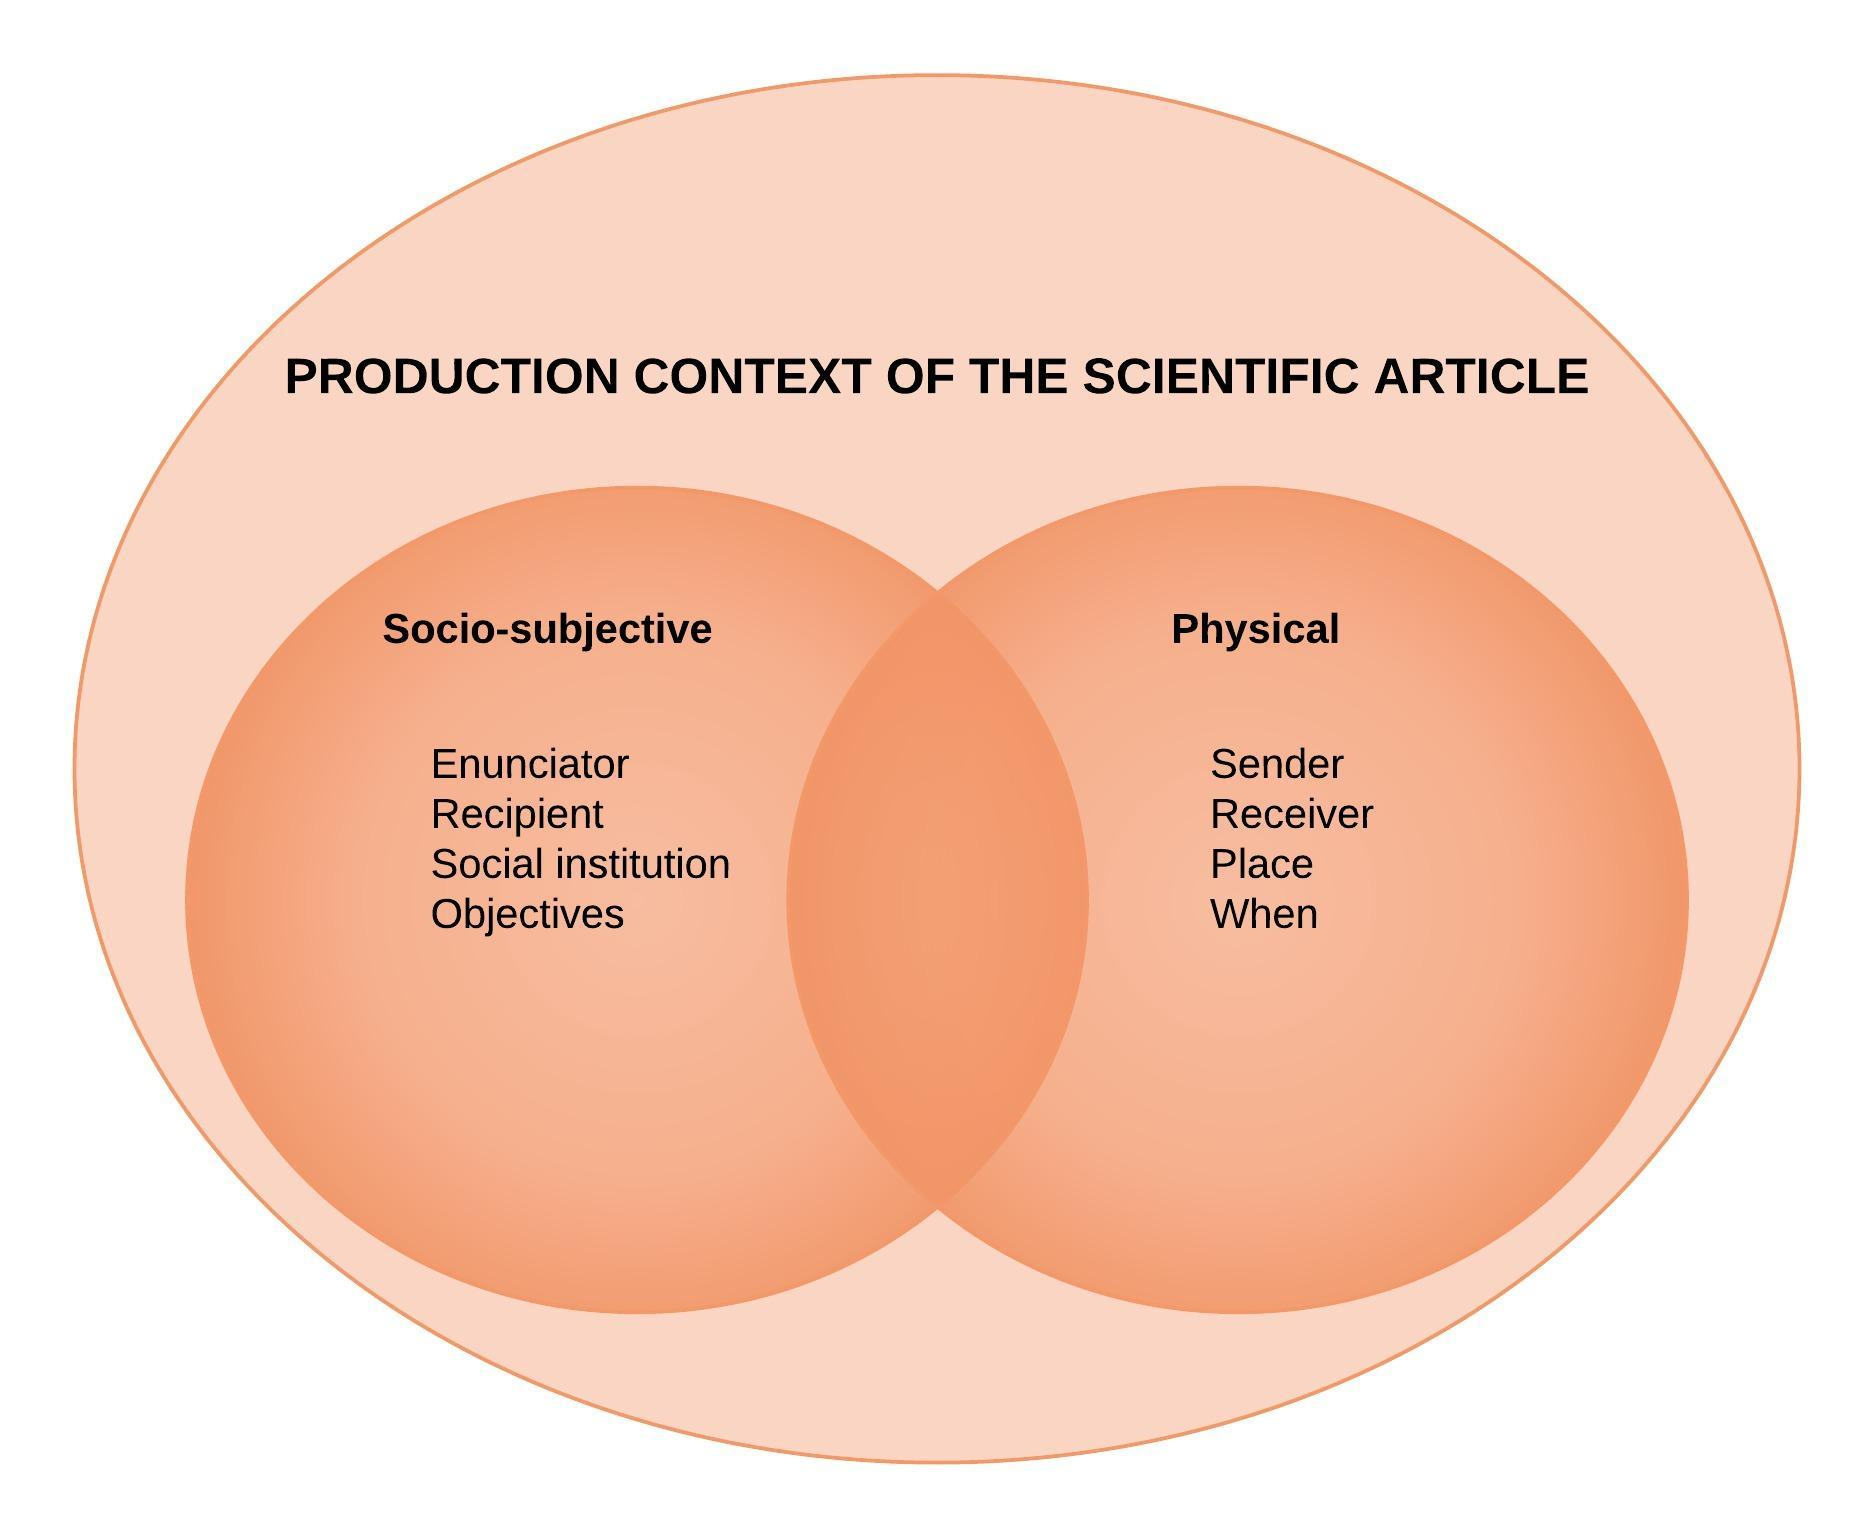
\includegraphics[width=0.85\textwidth]{Fig1.png}
 \caption{Planificação do contexto de produção do artigo científico.}
 \label{fig-01}
 \source{Adaptado do modelo de análise de textos de \textcite{bronckart_atividade_1999}.}
\end{figure}

O primeiro nível da infraestrutura textual ou contexto de produção é o mais profundo e é constituído pelo plano geral que se refere à organização do conjunto de conteúdo temático. Nesse contexto, \textcite[p. 97/98]{bronckart_atividade_1999} considera que “trata-se de conhecimentos que variam em função da experiência e do nível de desenvolvimento do agente e que estão estocados e organizados em sua memória, previamente, antes do desencadear da ação de linguagem”. Sendo assim, o conteúdo temático de um texto são as representações construídas pelo agente-produtor do texto, baseadas tanto no mundo físico e real quanto no mundo sociossubjetivo desse. Ademais, deve-se considerar o lugar e o papel social ocupado pelo produtor, assim como o momento histórico da produção e a posição social do receptor. Por exemplo, o plano geral de um artigo científico, geralmente, é constituído por: introdução, pressupostos teóricos, metodologia, resultados das análises e conclusões, sendo que cada uma dessas seções tem seus conteúdos e objetivos específicos.

Entre suas principais características estão a estrutura composicional e o estilo da textualização, visto que seu público é um grupo de especialistas na área, conhecedor do assunto, métodos e interesse na pesquisa divulgada. Assim, essas características são decisivas na construção do texto, ou seja, na superestrutura do artigo científico, assim como a seleção lexical das estruturas sintáticas, isto é, na composição do estilo.

Em seguida, na \Cref{fig-02}, além da apresentação da composição da infraestrutura geral do artigo, é apresentado um modelo de planificação para análise do segundo nível organizacional do artigo científico referente à composição do estilo, ou seja, as capacidades linguístico-discursiva:

\begin{figure}[htbp]
 \centering
 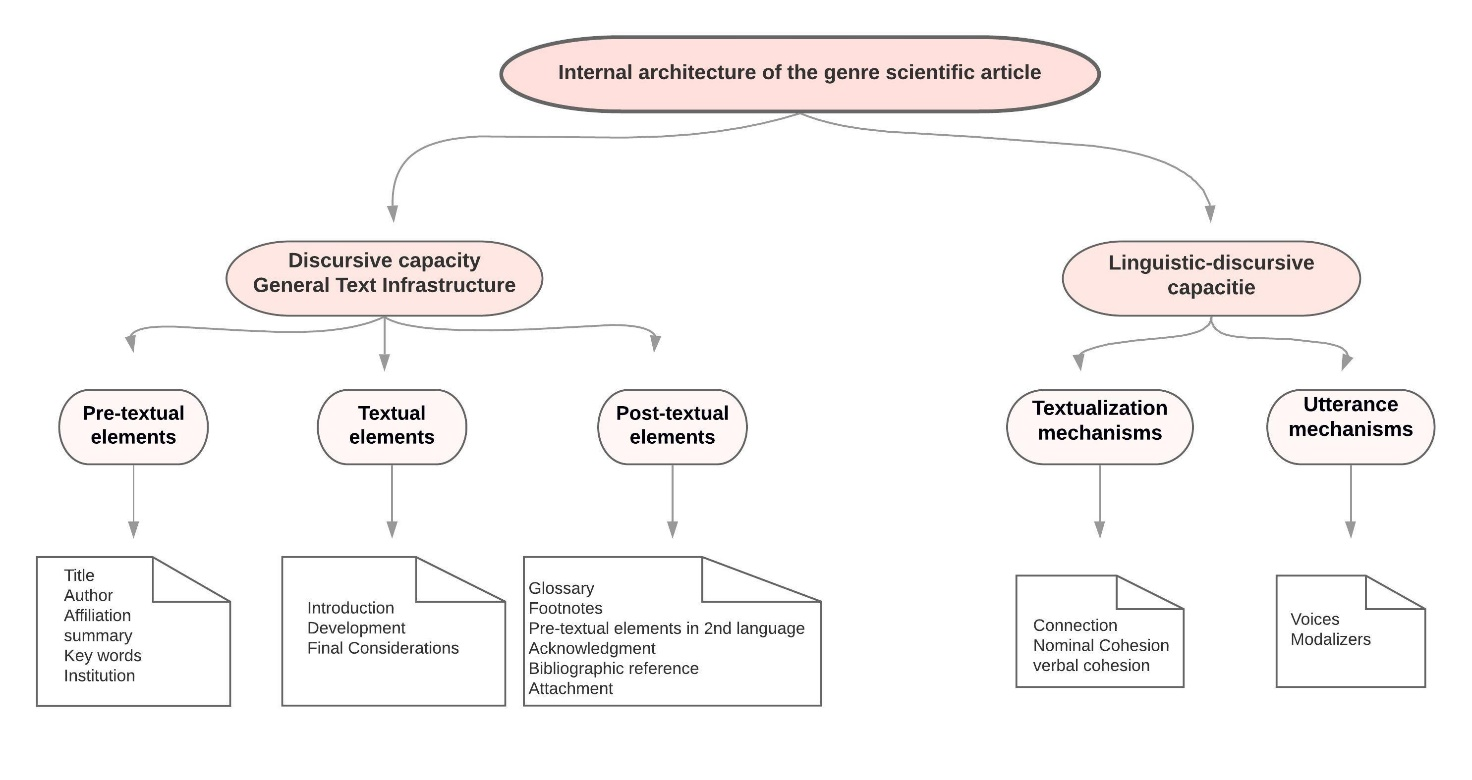
\includegraphics[width=0.85\textwidth]{Fig2.png}
 \caption{Planificação da Superestrutura do artigo científico.}
 \label{fig-02}
 \source{Adaptado do modelo de análise de textos de \textcite{bronckart_atividade_1999}.}
\end{figure}

A planificação da superestrutura do artigo científico representa o segundo nível organizacional e se refere aos mecanismos textuais, que, por sua vez, dividem-se em \textit{mecanismos de textualização} e\textit{mecanismos enunciativos}. A função desses mecanismos é contribuir para dar ao texto sua coerência linear ou temática, tornando explícitas as grandes articulações hierárquicas, lógicas, temporais e espaciais.

Os mecanismos de textualização garantem a conexão, a coesão nominal e a coesão verbal. Já os mecanismos enunciativos garantem a progressão do "conteúdo temático", dizem respeito às vozes assumidas no interior do texto e as modalizações avaliativas que compõem o enunciado. \textcite{bronckart_atividade_1999} afirma que:

\begin{quote}
    qualquer que seja a diversidade e a heterogeneidade dos componentes da infra-estrutura de um texto empírico, ele constitui um todo coerente, uma unidade comunicativa articulada a uma situação de ação e destinada a ser compreendida e interpretada como tal por seus destinatários. Essa coerência geral procede (...) dos mecanismos de textualização e (...) dos mecanismos enunciativos \cite[p. 259]{bronckart_atividade_1999}.
\end{quote}

Segundo \textcite{silva_elaboracao_2014}, muitos estudiosos, como \textcite{schneuwly_generos_2004}, retomam o modelo de \textcite{bronckart_atividade_1999}, para fins didáticos, ressaltando que, antes de o gênero ser levado para a sala de aula, é necessário que seja feito o seu modelo didático. Entretanto, as autoras salientam que existe uma diversidade de mecanismos que norteiam a elaboração desse modelo, sintetizados em três princípios de legitimidade, pertinência e solidarização. Para as autoras, esses princípios relacionados às capacidades de reconhecimento da infraestrutura textual e dos mecanismos de textualização podem servir de subsídios para a criação de um modelo didático do gênero artigo científico a fim de subsidiar professores e alunos de pós-graduação \textit{stricto sensu} a desenvolverem atividades para se apropriarem desse gênero.

Assim como na pós-graduação, esses princípios relacionados às capacidades de reconhecimento da infraestrutura textual e dos mecanismos de textualização podem servir de subsídios para a criação de um modelo representativo do gênero artigo científico a fim de subsidiar as aplicações no processamento automático de texto por meio da criação de marcações que recuperam as características próprias desse gênero.

\subsubsection{Planificação da representação em linguagem de marcação do gênero artigo científico}\label{sec-organizacao-latex}
É demonstrado na \Cref{fig-03} o modelo estrutural em forma de árvore com marcações em XML dos principais elementos constitutivos da representação da superestrutura do artigo científico. Esses elementos podem influenciar no armazenamento, na organização e na recuperação da informação no processamento automático do gênero:

\begin{figure}[htbp]
 \centering
 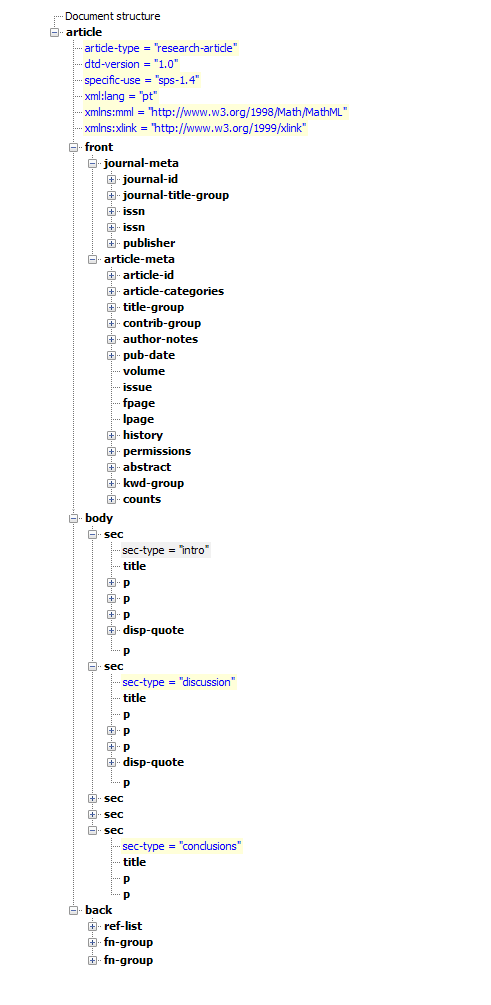
\includegraphics[width=0.5\textwidth]{Fig3.png}
 \caption{Modelo estrutural em forma de árvore dos principais elementos constitutivos da representação da superestrutura do artigo científico.}
 \label{fig-03}
 \source{Adaptado pela autora do banco de dados da SciELO.}
\end{figure}

Por meio da \Cref{fig-03}, pode-se observar que a estrutura básica do gênero artigo científico é representada pelo nó raiz (<article>) e este possui como filiação mais três nós, representativos de elementos pré-textuais (<front>), elementos textuais (<body>) e elementos pós-textuais (<back>).  Os elementos pré-textuais do <front> são caracterizados e descrevem os metadados do periódico, título, autoria, afiliação, resumo, palavras-chave, DOI, volume, número, suplemento, paginação, indicação da licença Creative Commons, data de publicação, seção de cabeçalho, histórico de datas, dados de correspondência, notas de autor, informações de resenhas de livros, contagem de elementos e dados de financiamento (se houver). Os elementos textuais do <body> são caracterizados e descrevem o corpo textual do artigo que pode ser constituído por seções. Cada uma delas possui um elemento <title> seguido de um ou mais parágrafos <p>. Seções de primeiro nível podem ser qualificadas de acordo com seu tipo por meio do atributo @sec-type, cujos valores possíveis, segundo o Guia de uso de elementos e atributos XML para documentos que seguem a implementação \textcite{Scielo}, são os constantes da \Cref{tbl02}.

\begin{table}[htbp]
\begin{center}
\caption{Tipo de seções.}
\label{tbl02}
\begin{tabular}{ll}
\hline 
\textbf{Valor}        & \textbf{Descrição}                                    \\
\hline
Cases        & Relatos/estudos de caso                             \\
Conclusions  & Conclusões/considerações finais/Final Remarkes \\
Discussion   & Discussões                                    \\
Introduction & Introdução/sinopse                          \\
Materials    & Materiais                                 \\
Methods      & Metodologia/método                           \\
Results      & Resultados                                        \\ \hline
\end{tabular}
\end{center}
\source{Guia de uso de elementos e atributos XML para documentos que seguem a implementação \cite{Scielo}.}
\end{table}

Os elementos pós-textuais do <back> são caracterizados e descrevem a parte final do documento que compreende lista de referências e demais dados referentes à pesquisa como: notas de rodapé, agradecimentos, apêndice, material suplementar, anexos e glossário.

A representação do modelo didático do artigo científico, em formato arbóreo, permite acrescentar aos dados linguísticos brutos informações sobre as características e a visualização das dimensões constitutivas do gênero, delimitar os objetivos a serem atingidos em relação aos diferentes propósitos de uso do texto no processamento automático. O enriquecimento do corpus com informações da composição do gênero, na forma de representações arbóreas em que se indicam as relações entre elementos do contexto de produção (constantes dos nós <front>  <article-meta> </article-meta> </front>), ou sentenças ou fragmentos de sentenças da infraestrutura geral do texto que podem aplicar qualquer formalismo estrutural imposto pelo XML de origem (compreendidos em <body> <sec> </sec> </body> e  <back> <ref-list> </ref-list> </back>) atribuído ao gênero.  Essa configuração em que consiste na transformação do texto puro em texto estruturado, indica as principais características do gênero que podem ser usadas em aplicações da linguística computacional, ou seja, no pré-processamento automático para resolver um dado problema ou auxiliar em uma dada atividade de localização, armazenamento e/ou recuperação da informação.

Acredita-se que, a partir da estrutura representativa de determinado gênero textual, é possível organizar e preparar a recepção e interpretação de determinados conteúdos para o processamento automático do texto. O pré-processamento de um gênero vai ser, de alguma forma, influenciado pelo reconhecimento da superestrutura e da infraestrutura de sua organização composicional.

Sendo assim, a construção e disponibilidade de bancos de árvores que representem os recursos de linguagem constitutivos do gênero textual é fundamental para fomentar as variadas aplicações em PLN. Essas informações estruturadas são importantes, pois sinalizam o contexto de produção e alguns organizadores textuais centrais que podem se revelar boas estratégias para o pré-processamento. Além disso, constituem bases de dados sobre os quais se pode efetuar análises qualitativas e quantitativas por variadas técnicas, que podem complementar outras abordagens.

\subsection{Trabalhos correlatos}\label{sec-titulo}
Alguns anotadores textuais disponíveis para análise fazem uso de abordagens complexas para a categorização de seus recursos de dados e exploração de correspondência para seus padrões. Dentre elas, as mais utilizadas são: a abordagem morfossintática que especifica o modo como os grupos de elementos devem se organizar; e, a abordagem semântica que especifica o que o grupo de elementos deve significar. A seguir, serão apresentadas as ferramentas computacionais eDictor, Aelius e COMEDI para anotação e processamento de texto, que utilizam abordagens morfossintática e semântica.

\subsubsection{eDictor}\label{sec-autores}

O eDictor\footnote{Disponível em: \url{https://humanidadesdigitais.org/edictor/}. Acesso em: 19 de abr. 2018.} é uma ferramenta utilizada para auxiliar a edição eletrônica em XML de textos antigos para fins de análise filológica e a codificação linguística automática \cite{sousa_o_2014}. Essa ferramenta foi idealizada para a criação do \textit{Corpus} Anotado do Português Tycho Brahe\footnote{Disponível em: \url{http://www.tycho.iel.unicamp.br/corpus/}. Acesso em: 19 de abr. 2018.} (CTB), cujas  principais funcionalidades são: I) flexibilidade dos formatos gerados, permitindo tanto a leitura humana como a leitura automática; II) garantia da qualidade filológica da edição por se tratar de um editor especializado; III) possibilidade de operar com vários níveis de edição: IV) Junção, Segmentação, Grafia, Modernização, Expansão, Correção, Pontuação; V) possibilidade de criar novos níveis de edição de acordo com a necessidade do pesquisador.

Dentre seus vários níveis de edição, destacam-se suas principais funcionalidades que são: junção e segmentação. A primeira é utilizada para unir trechos do texto como palavras quebradas, enquanto a segunda faz o oposto, separa trechos indevidamente unidos. Tais edições são feitas com anotação XML de forma a manter o texto original disponível para consulta. Essas edições nos textos podem incluir outros níveis de trabalho como modernização, expansão, grafia e pontuação \cite{sousa_o_2014, sousa_e-dictor:_2010, sousa_uma_2016}.

\subsubsection{Aelius}\label{sec-idioma}
O etiquetador Aelius\footnote{Disponível em: \url{http://aelius.sourceforge.net/}. Acesso em 19 de abr. 2018.} é um \textit{software} livre em desenvolvimento, para análise superficial do Português Brasileiro, que faz parte do projeto \textit{Aelius Brazilian Portuguese POSTagger}\footnote{Disponível em: Aelius Brazilian Portuguese Pos-tagger - \url{http://sourceforge.net/projects/aelius/files/}. Acesso em 19 de abr. 2018.} e está registrado no SourceForge.net\footnote{Disponível em: Sourcefoge.Net - Maior hospedagem mundial de software de código aberto. \url{http://sourceforge.net/}. Acesso em 19 de abr. 2018.} \cite{alencar_aelius:_2010, alencar_aelius_2013a, alencar_aelius_2013b}. Por possuir uma arquitetura híbrida, recorre às abordagens baseadas em regras formuladas manualmente e ao sistema estatístico estocástico baseado em n-gramas. O Aelius foi projetado para etiquetar morfologicamente textos escritos de maneira automática. Para tanto, esse editor desempenha as seguintes tarefas: I) pré-processamento de corpora; II) construção de \textit{language models} e etiquetadores com base num corpus anotado; III) avaliação do desempenho de um etiquetador; IV) comparação entre diferentes anotações de um texto; V) realização de anotação de \textit{corpora} e auxílio na revisão humana de anotação automática.

Essa ferramenta também inclui recursos de idioma, como modelos de linguagem, textos de amostra e padrões de ouro\footnote{Em PLN “padrão de ouro” significa que as avaliações mais fortes e significativas são baseadas em resultados do mundo real, em que um sistema é implantado operacionalmente e é medido seu impacto nos resultados gerados por usuários do mundo real \cite{reiter_structured_2018}.}. Atualmente, a Aelius já oferece recursos para \textit{corpora} e corporação de POS e gera anotações em diferentes formatos, como em XML no esquema de codificação TEI\footnote{Text Encoding and Interchange (TEI) define um conjunto vasto de elementos e atributos na linguagem XML que permitem representar características estruturais, conceituais e de visualização dos textos.} P5.

\subsubsection{COMEDI}\label{sec-resumo}
O \textit{COmponent Metadata EDItor} (COMEDI)\footnote{Disponível em: \url{http://clarino.uib.no/comedi/page?page-id=repository-main-page}. Acesso em 19 de abr. 2018.} é um editor de componentes para metadados baseado na Web, em conformidade com qualquer perfil CMDI\footnote{Component MetaData Infrastructure (CMDI), fornece uma estrutura para descrever e reutilizar um conjunto de metadados. Disponível em: \url{https://www.clarin.eu/content/component-metadata}. Acesso em 19 de abr. 2018.}, e que oferece suporte atualizado para recursos adotado pela CLARIN\footnote{Common Language Resources and Technology Infrastructure (CLARIN), é uma infraestrutura de pesquisa que foi iniciada a partir da visão de que todos os recursos e ferramentas de linguagem digital de toda a Europa e além são acessíveis através de um ambiente \textit{on-line} de \textit{logon único} para o apoio de pesquisadores nas ciências humanas e sociais. Disponível em: \url{https://www.clarin.eu/}. Acesso em 19 de abr. 2018.}. No COMEDI, é possível criar um registro de metadados a partir do zero, ou carregar, editar e baixar qualquer arquivo XML CMDI. Seus componentes poderem ser usados independentemente do editor, ou podem ser usados por meio de uma interface web, em que o usuário seleciona um perfil CMDI para iniciar, e o editor exibe o perfil como um formulário \textit{on-line} simples que oculta o código XML. Além disso, o editor pode funcionar como um servidor completo para armazenar, pesquisar, visualizar e gerenciar, por meio da administração de grupos e de usuários, o controle sobre o direito de acesso aos metadados individuais. O gerenciamento de usuários do editor é feito pela autenticação do \textit{login} e opera em dois níveis: o de usuário e o de grupo \cite{lyse_comedi:_2015}.

A Um perfil CMDI consiste em \textit{componentes} e \textit{elementos}. Os elementos são os nós terminais, nos quais são atribuídos um valor, digitado em um campo de texto do formulário, ou selecionado em um menu suspenso. Os elementos que pertencem aos terminais geralmente são agrupados em componentes, por exemplo, um componente pessoa (com elementos como sobrenome, nome) ou um componente licença (com elementos como nome da licença, URL da licença). Em resumo, os perfis recomendados, e que são encontrados no menu suspenso COMEDI, são: I) \textit{corpusProfile}: descreve \textit{corpora} de todos os tipos e modalidades; II) \textit{lexicalProfile}: descreve recursos lexicais; III) o usuário é livre para desenvolver o seu próprio perfil, mas nesse caso, deve reutilizar os componentes existentes, na medida do possível. Essas recomendações têm como objetivo auxiliar na descrição dos recursos linguísticos com metadados de acordo com a estrutura do CMDI. Para isso, o editor precisa distinguir campos obrigatórios de campos opcionais e impor que as entradas obrigatórias sejam preenchidas \cite{dima_metadata_2012}.

As ferramentas computacionais eDictor, Aelius e COMEDI são utilizadas para anotação e processamento de texto, baseadas na utilização de abordagens morfossintática e semântica. Entretanto, não foi observada, nos anotadores analisados, a utilização do gênero textual como recurso de dado a ser explorado para anotação e processamento de texto, revelando a necessidade de uma abordagem discursiva.

Em seguida, será apresentado um modelo computacional que, por meio da abordagem discursiva, filtra e categoriza os recursos de dados contextuais do artigo científico, referente à sua construção composicional, demonstrando a relevância desse tipo de anotação para a compreensão e categorização de padrões do contexto de produção desse gênero. Segundo \textcite{cambria_jumping_2014}, trabalhos mais recentes reconhecem a necessidade de categorizar os recursos de linguagem que expressam o conhecimento externo do texto na interpretação e resposta à entrada de linguagem. Esse conhecimento está relacionado à abordagem \textit{pragmática} que especifica como as informações contextuais podem ser aproveitadas para fornecer melhor correlação entre as variadas abordagens (morfossintática e semântica) já existentes e combiná-las entre si.

\section{Modelo computacional – AnoTex}\label{sec-secoes}
O AnoTex\footnote{AnoTex - para a construção automática de \textit{corpus} partir do gênero do texto-base. Ferramenta computacional versão 0.1 beta, linha de comando, escrita em ANSI C, desenvolvida para funcionar em qualquer sistema que disponha de uma libc, contém bibliotecas para extração de informações disponíveis em formato XML e PDF, além de serviços disponíveis para consulta e ampliação \cite{fonseca_2018}.} é um anotador textual em desenvolvimento, cuja principal funcionalidade é extrair as características constitutivas do gênero artigo científico por meio das marcações em XML enriquecidas com informações linguísticas sobre sua construção composicional \cite{fonseca_etal_2018}. Sua principal atribuição é processar os elementos do contexto de produção e da infraestrutura geral do texto, para a compilação do corpus de estudo. Essa ferramenta é capaz de filtrar e exportar os elementos anotados em XML e do seu PDF relacionado, extraídos de banco de dados disponíveis na web, como por exemplo da Biblioteca Eletrônica SciELO-\textit{Scientific Electronic Library On-line}\footnote{Disponível em: \url{http://www.scielo.br}. Acesso em 12 jan 2018.}.

O conjunto de aplicações desempenhado pelo AnoTex está demonstrado na \Cref{fig-04} que, em síntese, corresponde ao delineamento do modelo computacional adequado aos propósitos da pesquisa, dividido em quatro etapas denominadas: 1 seleção, 2 compilação, 3 processamento e 4 exportação dos dados.

\begin{figure}[htbp]
 \centering
 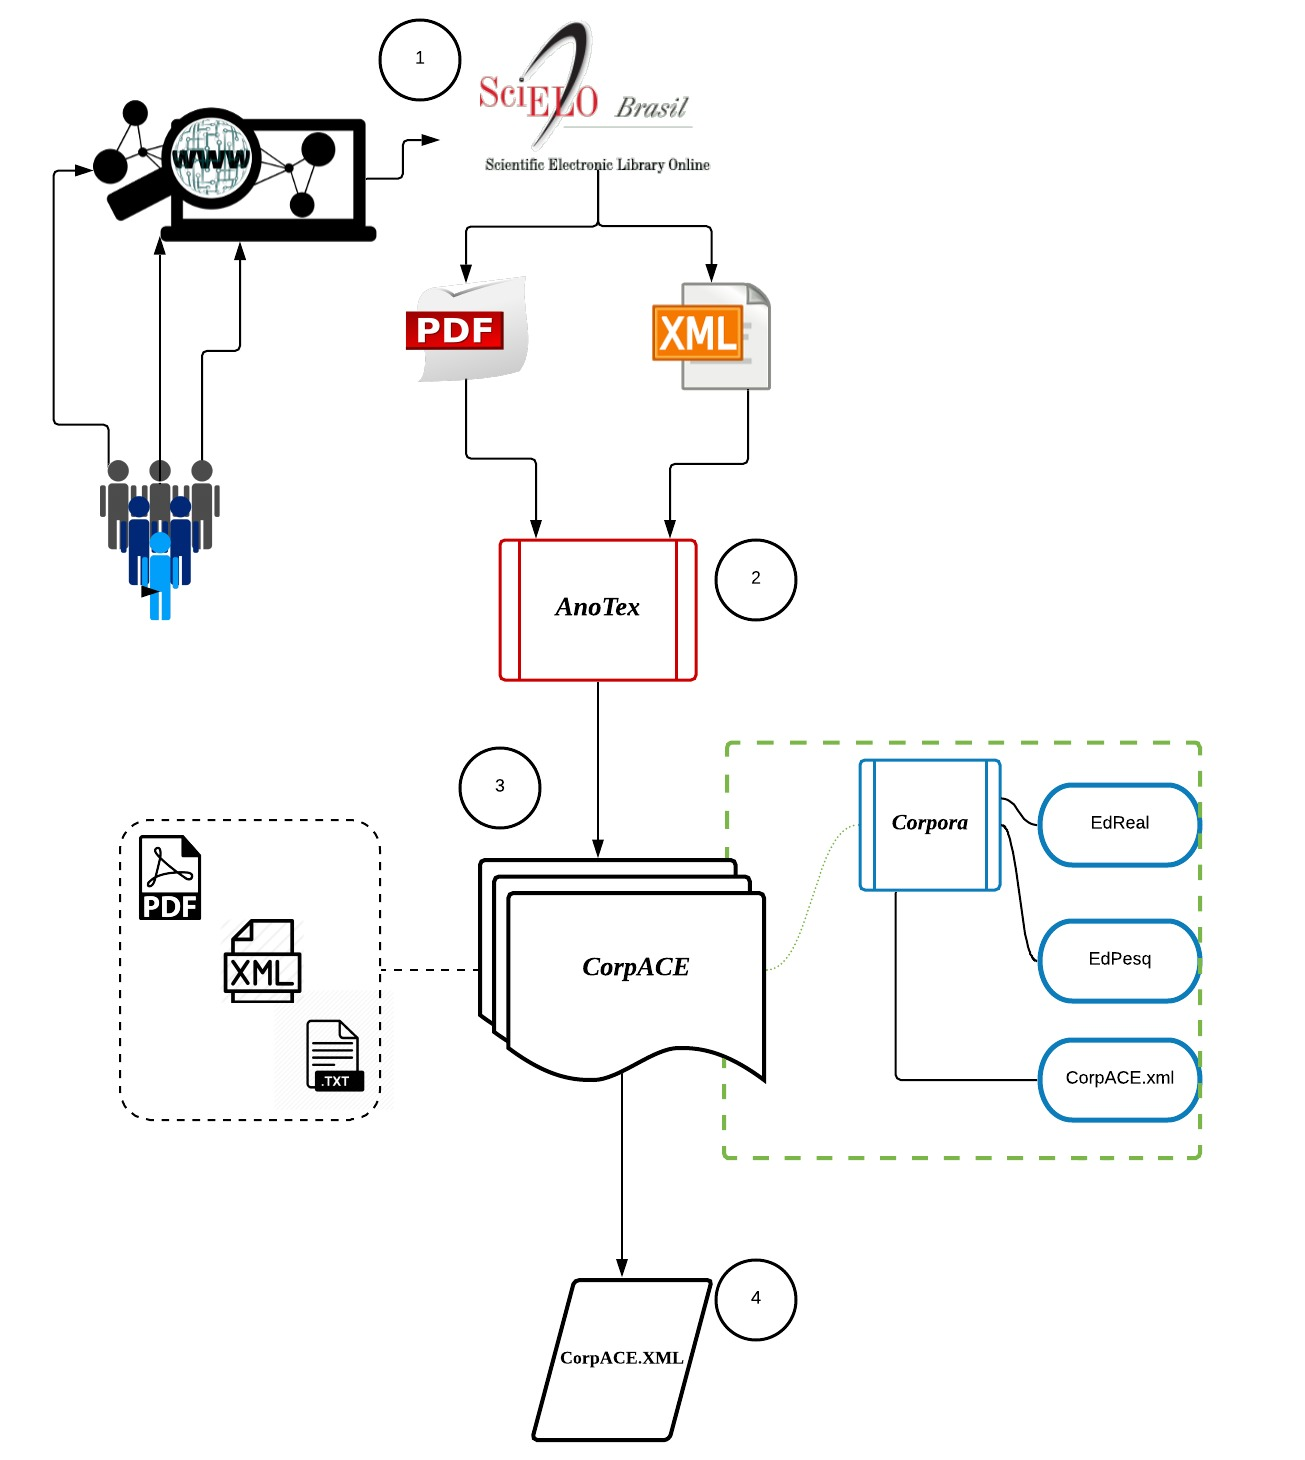
\includegraphics[width=0.85\textwidth]{Fig4.png}
 \caption{Modelo de compilação do AnoTex.}
 \label{fig-04}
 \source{\cite{fonseca_etal_2018}.}
\end{figure}

As três primeiras etapas ilustradas no modelo dizem respeito à qualidade dos dados, sendo elas:

\begin{enumerate}
    \item \textit{Seleção}: Escolha do conjunto de requisitos do gênero artigo científico, enfatizado pelo uso de etiquetas XML, necessário para impactar na validade e confiabilidade do corpus de análise, adequando-o aos propósitos da investigação, isso é, que permita destacar as características e a visualização das dimensões constitutivas do gênero;
    \item \textit{Compilação}: Captura do conjunto ou amostra de dados constitutivos do gênero textual a serem manipulados. Em outras palavras, é nessa etapa que são organizados e gerados os corpora compostos de corpus com características específicas para a análise desejada;
    \item \textit{Processamento}: Transformação e/ou tratamento dos dados, tais como ruídos, inconsistências, dados inexistentes ou incompletos, que podem gerar padrões distorcidos, eliminação de atributos redundantes, padronização do conjunto de valores dos elementos selecionados dos artigos.
    Atualmente, o AnoTex filtra 06 elementos pré-textuais, compreendidos no <front> com categorização e marcação com informações sobre: Nome da revista: <journal-title> </journal-title>; Título do artigo: <article-title> </article-title>; Nome do autor: <contrib contrib-type="author"> <name> <surname> </surname> <given-names> </given-names> </name>; Instituição: <institution content-type=""> </institution>; Resumo:<abstract> <title></title> </abstract>; Palavras-Chave: <kwd-group xml:lang=""> <title> </title> <kwd></kwd> </kwd-group>.
Dentre os elementos textuais, compreendidos no <body>, são filtradas as seções e subseções com categorização de marcações com informações sobre: Introdução: <sec sec-type="intro"> <title></title> </sec>; Desenvolvimento: <sec sec-type="discussion"> <title></title> </sec>; Considerações finais: <sec sec-type="conclusions"> <title></title> </sec>.
Além disso, o AnoTex filtra as referências bibliográficas dos elementos pós-textuais, compreendidos no <back> com categorização e marcação com informações sobre: Referências bibliográficas: <ref-list> <title> </title> <ref> </ref> </ref-list>;
    \item \textit{Exportação}: Saída do corpus em um arquivo XML, para interpretação e avaliação dos padrões identificados em função dos objetivos iniciais. Estas etapas convergem para a formação de uma base de dados concisa, em que dados de diferentes periódicos sejam coletados e armazenados em um único conjunto de dados.
\end{enumerate}

A \Cref{fig-05}, a seguir, apresenta uma amostra da configuração do \textit{CorpACE} gerada pelo AnoTex. Os elementos pré-textuais demonstrados em 1, 2, 3, 4 5, 8 e 10 correspondem a representação do contexto de produção; os elementos textuais demonstrados em 6 e 9 correspondem a representação da arquitetura geral do texto, assim como os elementos pós-textuais demonstrados em 7.

\begin{figure}[htbp]
 \centering
 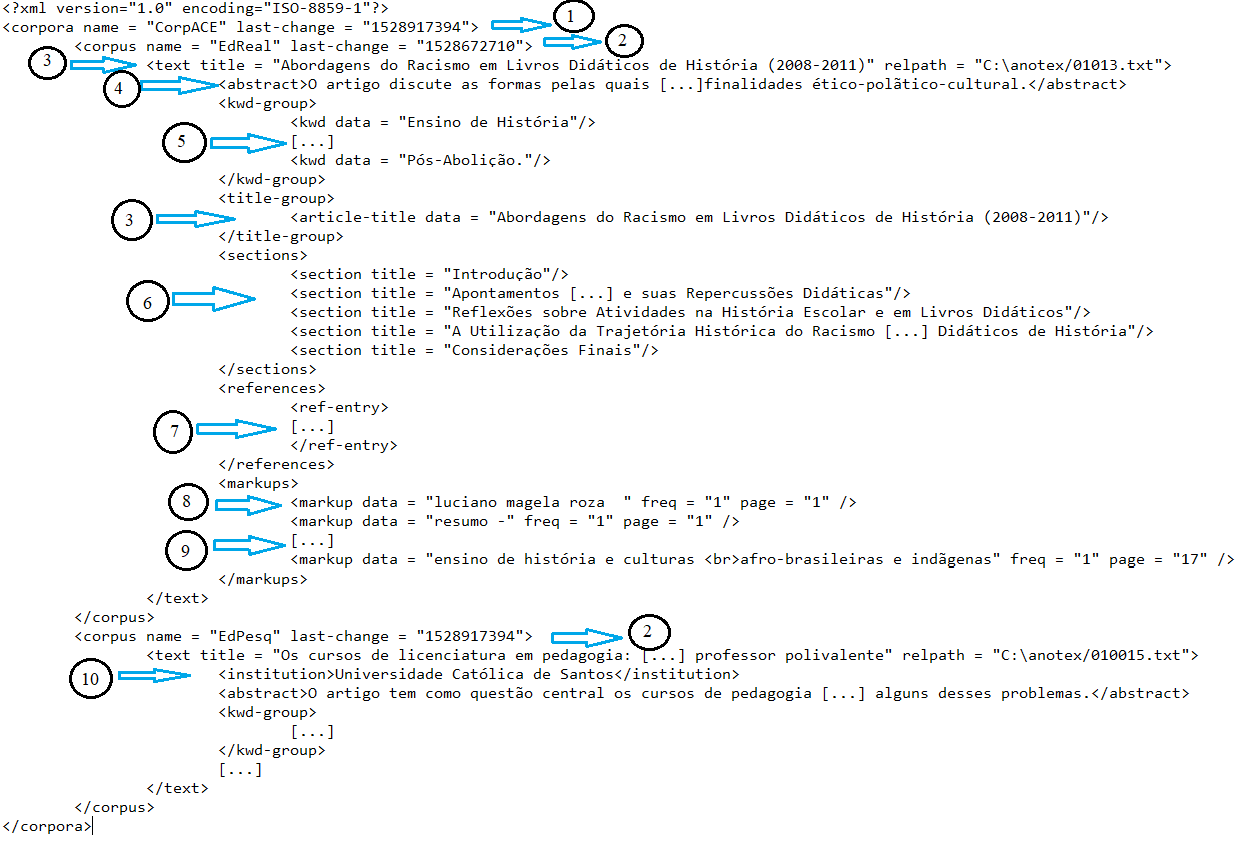
\includegraphics[width=0.85\textwidth]{Fig5.png}
 \caption{Amostra da configuração do \textit{CorpACE}.}
 \label{fig-05}
 \source{Adaptado pela autora do AnoTex v0.1b.}
\end{figure}

Por meio da \Cref{fig-05}, pode-se observar que após a filtragem de cada elemento, o AnoTex cria o \textit{CorpACE} gerando um arquivo de saída XML (baseado na entrada dos dados do XML e do PDF). Essa base textual servirá para análise linguística, treinamento e análise de ferramentas computacionais cuja finalidade seja o processamento de texto. A separação entre a estrutura e apresentação dos dados dão maior maleabilidade à informação (a partir de um mesmo XML é possível apresentar a informação de formas distintas além de carregar metadados em uma base de dados). Os dados representados pelo XML são estruturados de forma arbórea, e cada tag ou marca representa um nó ou elemento na árvore.

Para a saída dos corpora em um arquivo XML, o AnoTex precisou receber cinco argumentos obrigatórios: o arquivo em PDF, o arquivo XML, a denominação dos corpora, a denominação do arquivo de saída e em qual corpus, desse arquivo de saída, a marcação foi adicionada. Uma vantagem, desse processo, é que um arquivo XML de saída pode reunir diversos corpora, requisito muito útil se, por exemplo, for necessária a criação de diferentes versões do mesmo corpus. O AnoTex permite a criação de vários corpora, adicionados dentro do mesmo arquivo, esse conjunto de requisito constitui os corpora do arquivo. Todas essas funcionalidades puderam ser visualizadas nas \Cref{fig-04} e \Cref{fig-05}.

\section{Resultados e discussão}\label{sec-format-simple}
Para obter os resultados, foram utilizados 87 artigos de Qualis A1\footnote{O Qualis constitui-se um sistema brasileiro de avaliação de periódicos, mantido pela CAPES (Coordenação de Aperfeiçoamento de Pessoal de Nível Superior). Relaciona e classifica os veículos utilizados para a divulgação da produção intelectual dos programas de pós-graduação "\textit{stricto sensu}" (mestrado e doutorado), quanto ao âmbito da circulação (local, nacional ou internacional) e à qualidade (A, B, C), por área de avaliação. Os estratos estão divididos em 8 níveis, em ordem de qualidade.}, publicados pelas revistas “Educação \& Realidade”\footnote{Disponível em: \url{http://www.seer.ufrgs.br/index.php/educacaoerealidade/index}. Acesso em 12 jan 2018.} e "Educação e Pesquisa"\footnote{Disponível em: \url{http://www.educacaoepesquisa.fe.usp.br/}. Acesso em 12 jan 2018.}, no ano de 2017.  Os artigos foram coletados do \textit{site} SciELO e gravados em arquivos individuais no formato PDF, XML e TXT, formatos que são suportados pelo AnoTex. A compilação desses arquivos gerou o \textit{CorpACE} que é caracterizado como \textit{corpora} especializados, uma vez que são compostos por textos de uma única área de especialidade: Ensino e representativo de um único gênero textual, o artigo científico. Conforme esquematização de \textcite{sardinha_linguistica_2004}, quanto ao tamanho, os \textit{corpora} se enquadram como de médio porte. Em seguida, apresentamos a \Cref{tbl03} com os principais dados numéricos que caracterizam o \textit{CorpACE}:

\begin{table}[htbp]
\begin{center}
\caption{Resultados estatísticos do \textit{CorpACE}.}
\label{tbl03}
\begin{tabular}{ll}
 \toprule 
\textbf{Estatísticas}         &        \textbf{Total} \\ \hline                          \\
Número de artigos         &         87                              \\
Total de palavras   &                 750380                          \\
Número de palavras do menor artigo    &  6144                            \\
Número de palavras do maior artigo  &     18758                           \\
Número médio de palavras por artigo          &         8625               \\
Número de palavras filtradas dos elementos constitutivos do gênero    &   130128 \\
Número de palavras do \textit{Corpus} EdReal     &  383506                             \\
Número de palavras do \textit{Corpus} EdPesq   &     366874                            \\ \hline 
\end{tabular}
\end{center}
\source{Elaborada pelos autores.}
\end{table}

O \textit{CorpACE} foi submetido a um tratamento computacional possibilitado pela LC, que se faz presente metodologicamente, nesta pesquisa, por meio da ferramenta AnoTex que gerou os dados da \Cref{tbl03}. Foram utilizadas duas bibliotecas principais da ferramenta para a filtragem dos dados em XML e do PDF dos arquivos dos artigos.  A primeira foi utilizada para organizar os \textit{corpora} em bancos de árvore com informações do contexto de produção e da infraestrutura geral do texto. A segunda foi utilizada para obter dados das expressões em negrito e itálico com informações estatísticas de localização e frequência nos textos.  A ferramenta ajudou tanto na organização dos dados como na análise dos elementos mais frequentes utilizados nos artigos científicos.

O \textit{CorpACE} é constituído por três \textit{corpora}, que possuem um total de 750380 palavras, distribuídas em 87 artigos científicos. Esses \textit{corpora} estão assim subdivididos: \textit{corpus} EdReal (Revista Educação e Realidade), com 383505 palavras distribuídas em 45 artigos científicos; \textit{corpus} EdPesq (Revista Educação e Pesquisa) com 366874 palavras distribuídas em 42 artigos científicos; e \textit{corpus} CorpACE.xml com 130128 palavras dos elementos filtrados (EF) dos 87 artigos.

O primeiro passo para a análise dos dados levantados é, no arquivo XML gerado na saída do AnoTex, observar e realizar a organização e sistematização do resultado das marcações dos elementos constitutivos do gênero que foram selecionados e especificados na etapa 3 de processamento.

Em seguida, feitas as delimitações de cada \textit{corpus} apresentamos a contagem e a sistematização dos \textit{corpora} EdReal e EdPesq, por elemento filtrado, separadamente na \Cref{fig-06}.

\begin{figure}[htbp]
 \centering
 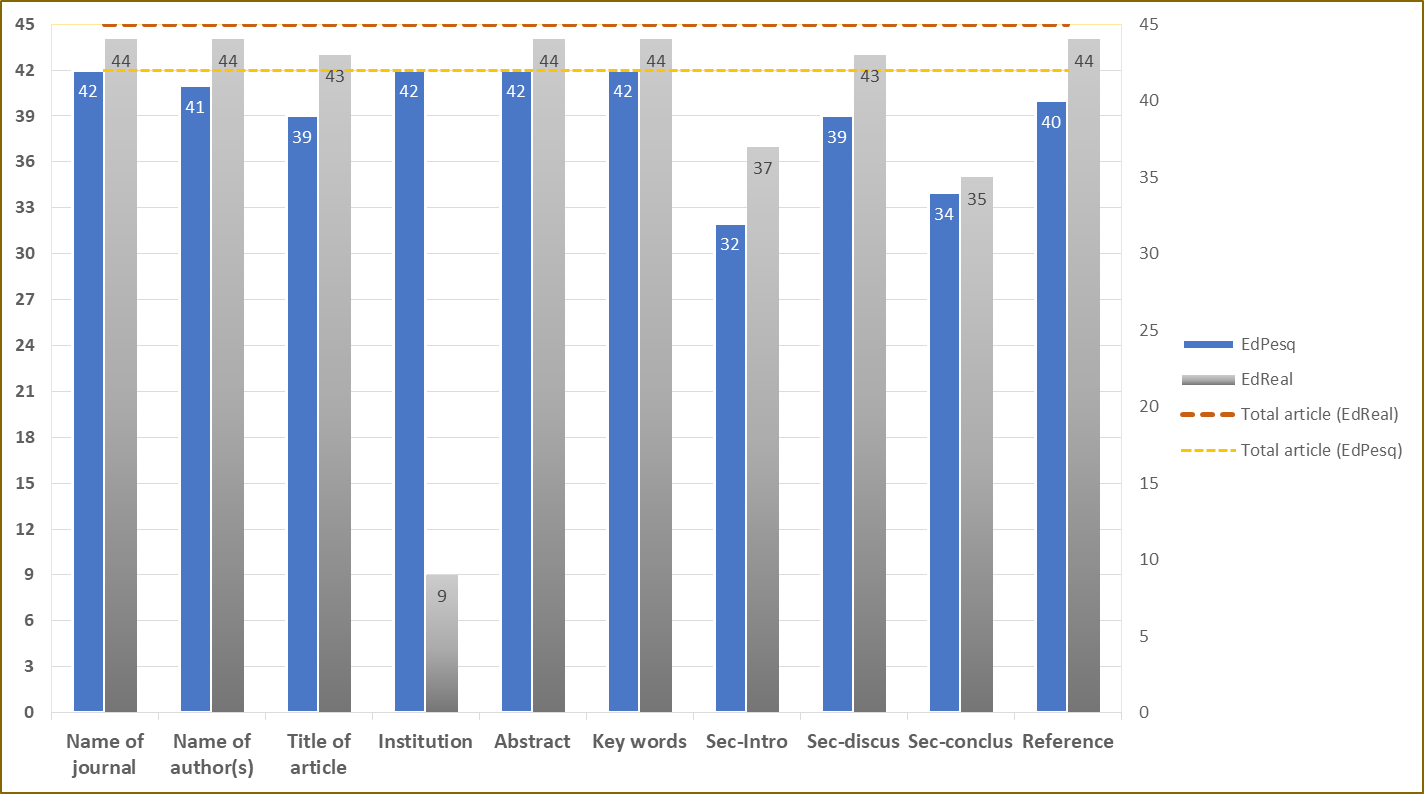
\includegraphics[width=0.85\textwidth]{Fig6.png}
 \caption{Elementos filtrados por \textit{corpus}.}
 \label{fig-06}
 \source{Elaborado pela autora.}
\end{figure}

Na \Cref{fig-06}, são mostradas as quantidades de elementos que foram filtradas dos artigos científicos de cada \textit{corpus}. Os resultados apontam que a ferramenta AnoTex conseguiu filtrar os elementos constitutivos do gênero dos 42 artigos selecionados, da Revista EdPesq, nas seguintes proporções:

\begin{itemize}
    \item \textit{Elementos do <fornt>}: Nome da Revista 100\%; Nome Autor(es): 97,6\%; Título do Artigo: 92,9\%; Instituição: 100\%; Resumo: 100\%; Palavras-Chave: 10\%;
    \item \textit{Elementos do <body>}: Seção Introdução: 76,2\%; Seção Discussão: 92,9\%; Seção Conclusão: 81,0\%;
    \item \textit{Elementos do <back>}: Referência: 95,2\%. A filtragem dos elementos constitutivos do gênero textual, dos 45 artigos selecionados da Revista EdReal, gerou os seguintes resultados:
    \item \textit{Elementos do <fornt>}: Nome da Revista 100\%; Nome Autor(es): 100; Título do Artigo: 97,8\%; Instituição: 20,0\%; Resumo: 97,8\%; Palavras-Chave: 97,8\%;
    \item \textit{Elementos do <body>}: Seção Introdução: 82,2\%; Seção Discussão: 95,6\%; Seção Conclusão: 77,8\%;
    \item \textit{Elementos do <back>}: Referência: 97,8\%.
\end{itemize}

O resultado da filtragem do elemento Instituição <institution content-type=""> </institution> na Revista EdReal chamou a atenção em função da discrepância em relação à filtragem do mesmo elemento na Revista EdPesq. Essa alteração se deu em função de um problema na marcação da \textit{tag} <aff id="aff1">, por parte da revista, em que foi deixado um "I" solto no meio do código, confundindo o \textit{parsing} do AnoTex. Para resolver esse problema, o "I" foi envolvido com a marcação <label> I</label>, igualmente marcado nos outros arquivos que funcionaram, o que solucionou o problema e possibilitou a filtragem do dado (\Cref{fig-07} e \Cref{fig-08}).

\begin{figure}[htbp]
 \centering
 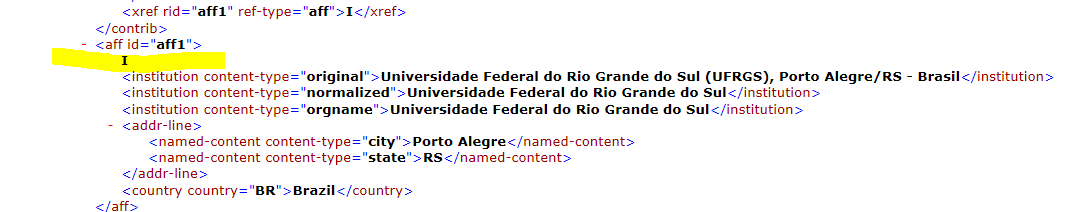
\includegraphics[width=\textwidth]{Fig7.png}
 \caption{Representação do código com problema na marcação.}
 \label{fig-07}
 \source{Adaptado pela autora do \textit{CorpACE}.}
\end{figure}

\begin{figure}[htbp]
 \centering
 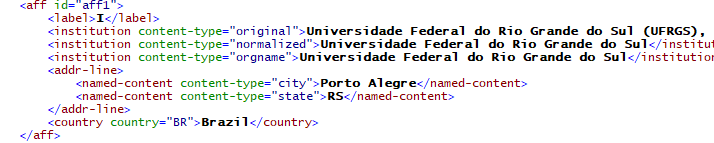
\includegraphics[width=0.85\textwidth]{Fig8.png}
 \caption{Representação do código sem problema e após correção.}
 \label{fig-08}
 \source{Adaptado pela autora do \textit{CorpACE}.}
\end{figure}

Embora tenha ocorrido essa discrepância na filtragem do elemento <institution>, em função de um problema na produção do XML, o resultado foi considerado, de um modo geral, satisfatório conforme demonstrado na \Cref{fig-09}.

\begin{figure}[htbp]
 \centering
 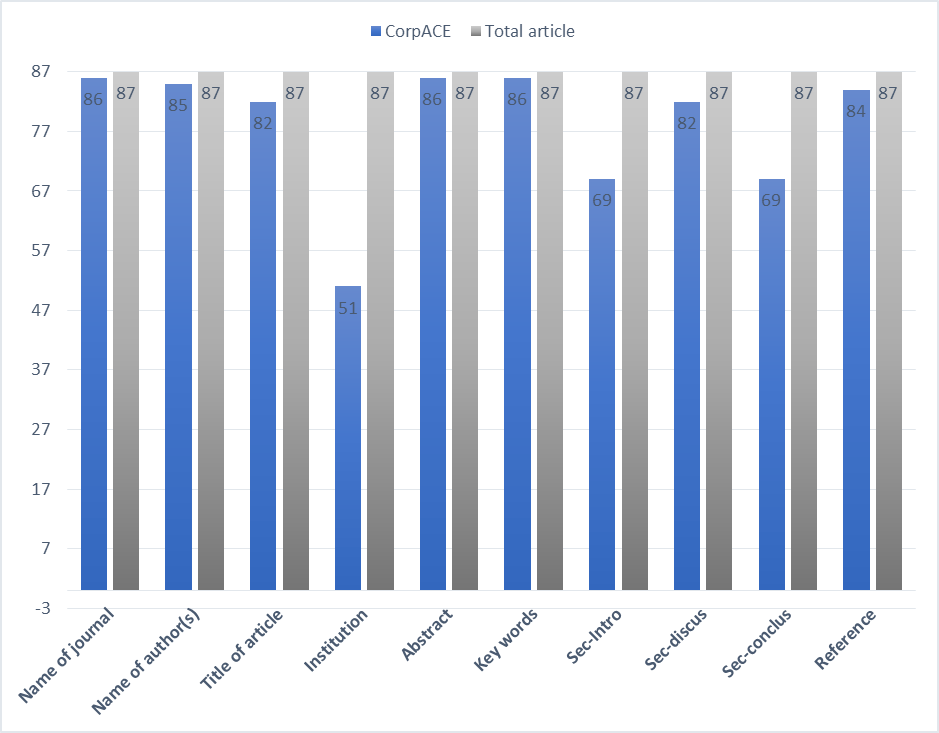
\includegraphics[width=0.85\textwidth]{Fig9.png}
 \caption{Total de elementos filtrados para o \textit{CorpACE}.}
 \label{fig-09}
 \source{Elaborado pela autora.}
\end{figure}

Na \Cref{fig-09}, são mostradas as quantidades de elementos que foram filtradas dos artigos científicos no total. Os resultados apontam que a ferramenta AnoTex conseguiu filtrar, pelo menos 4 e no máximo os 10 elementos representativos do gênero em todos os 87 artigos selecionados, nas seguintes proporções:

\begin{itemize}
    \item \textit{Elementos do <fornt>}: Nome da Revista: 100\%; Nome Autor(es): 98,9\%; Título do Artigo: 95,4\%; Instituição: 58,6\%; Resumo: 98,9\%; Palavras-Chave: 98,9\%;
    \item \textit{Elementos do <body>}: Seção Introdução: 79,3\%; Seção Discussão: 94,3\%; Seção Conclusão: 79,3\%;
    \item \textit{Elementos do <back>}: Referência: 96,6\%.
\end{itemize}

Ainda quanto à análise das distorções, outro elemento que chamou a atenção foi a marcação do título do artigo <article-title> </article-title>, embora todas as marcações com essa denominação tenham sido filtradas, foi considerado para o resultado apenas as que trouxeram a \textit{tag} e o conteúdo do texto (o título propriamente dito). Dos 87 arquivos analisados, em 04 deles a \textit{tag} </article-title> foi filtrada, mas o texto do título não. O que veio no lugar foi a expressão (null) em vez da informação sobre o título. Foi observado, nessas quatro amostras, que esses títulos estavam representados com caracteres diferentes do tipo parte em negrito ou nota de rodapé, por exemplo. O arquivo incluía uma \textit{tag} que confundia a lógica da filtragem. Segundo a lógica do AnoTex, como foi encontrada mais de uma \textit{tag}, uma nova indireção foi criada. Com isso, o título ficou situado num nível mais abaixo do qual deveria estar localizado.

Normalmente, seguindo as recomendações do guia de publicações da SciELO, o dado relevante do título, propriamente dito, fica no nível etiquetado como "article-title", conforme demonstrado na \Cref{fig10}.

\begin{figure}[htbp]
 \centering
 
\includegraphics[width=0.85\textwidth]{Fig10.png}
 \caption{Representação do Título.}
 \label{fig10}
 \source{Adaptado pela autora do \textit{CorpACE}.}
\end{figure}

Com a variação da marcação "bold" o título ficou em “article-title->bold->"o título"”. A \Cref{fig-11} ilustra a referida variação.

\begin{figure}[htbp]
 \centering
 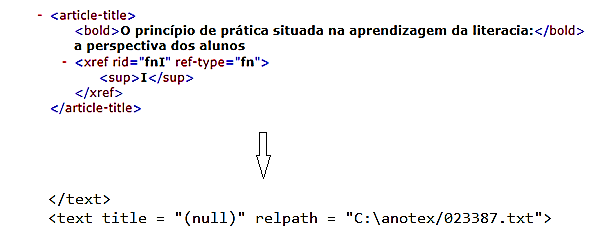
\includegraphics[width=0.85\textwidth]{Fig11.png}
 \caption{Título situado num nível mais abaixo do qual deveria ser.}
 \label{fig-11}
 \source{Adaptado pela autora do \textit{CorpACE}.}
\end{figure}

Esse arquivo mostra uma clara variação na anotação, por parte da revista, em relação às recomendações do \textcite{Scielo}. Nesse caso, foi concentrada muita informação onde deveria haver apenas uma, mais direta e valiosa, no caso o título na forma como nós humanos usaríamos para referenciar o artigo. Uma vez que essas marcações são feitas pelos profissionais da Revista, isso demonstra que o título deveria passar por uma normalização antes de ser \textit{tagueado}, pois permitiria maior aproveitamento do recurso de linguagem que está sendo disponibilizado. Para resolver esse problema, em específico, foi feita uma alteração para essa variação e caso o AnoTex achasse a \textit{tag} "bold" deveria ignorá-la. No caso ilustrado foi retirada a \textit{tag bold} (<bold> e </bold>) e o título voltou ser filtrado.

Outro recurso que demonstrou um pouco de variação em sua anotação foram os dados filtrados referentes aos elementos Sec-intro (seção introdução), Sec-discus (seção discussão), Sec-conclu (seção conclusão). Embora exista uma recomendação com as especificações no Guia de uso de elementos e atributos XML para documentos que seguem a implementação \textit{SciELO Publishing Schema}, Versão 1.5.1 \cite{Scielo}, conforme foi demonstrado na \Cref{tbl02} - Tipo de seções, os artigos não seguem um padrão estrito e homogêneo de formato para a marcação do corpo do texto <body>. Sendo assim, foi considerado para compor o resultado apenas os artigos que possuíssem seções com o atributo <sec-type> (\Cref{fig-12}).

\begin{figure}[htbp]
 \centering
 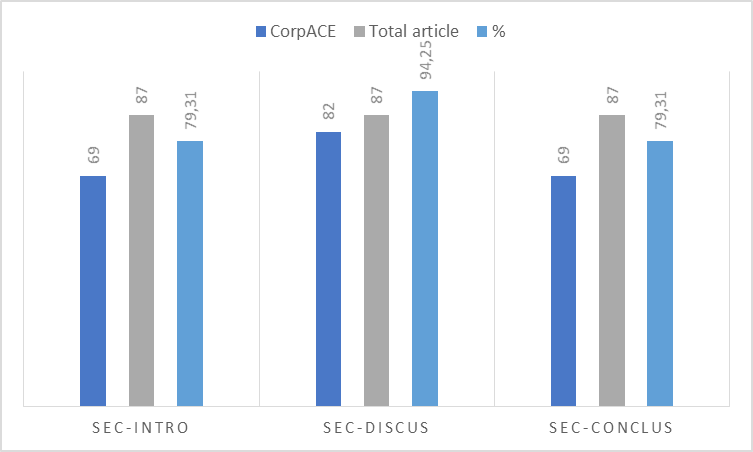
\includegraphics[width=0.85\textwidth]{Fig12.png}
 \caption{Filtragem dos elementos tipo de seção.}
 \label{fig-12}
 \source{Elaborado pela autora.}
\end{figure}

Seguindo essa especificação, os resultados demonstraram que, em uma das amostras analisadas, um dos artigos estava sem marcação para o atributo seção, e em outras amostras a marcação para esse atributo não conferia com as seções padrão que são caracterizadas conforme recomendação do Guia. Na filtragem desses elementos, foi observado que às vezes as seções de primeiro nível do artigo apresentavam o atributo  <sec-type> definidas pelo guia SciELO como: <sec sec-type="intro"> com 69 ocorrências; <sec sec-type="discussion"> com 82 ocorrências; e, <sec sec-type="conclusions"> com 69 ocorrências; às vezes vinham apenas com o atributo <sec> sem a especificação do tipo, com 17 ocorrências; e, às vezes não possuíam nenhuma marcação, todo o texto do artigo estava marcado apenas por parágrafos (isso foi observado em apenas uma amostra). Essa constatação possibilitou o entendimento de que o sistema de marcação de dados não obriga a existência do atributo \textit{sec/@sec-type}, ou seja, não é uma recomendação obrigatória para as revistas.

À medida que o uso das marcações em XML das seções dos artigos, foram analisadas para no processamento do texto, foram observadas algumas questões que confundiram a lógica do \textit{parsing} do AnoTex. Em uma amostra analisada, por exemplo, uma seção de primeiro nível que condiz com uma lista de valores próximos, obrigatoriamente apresentava um atributo \textit{@sec-type} e continha aninhadas dentro da seção de primeiro nível “introdução” as seções “discussão” e “conclusão”. Por serem, também, de primeiro nível as seções “discussão” e “conclusão”, pela lógica, não deveriam vir aninhadas dentro da seção “introdução”. Nesse caso, como o guia não recomenda esse tipo de marcação não foi possível para o AnoTex prever a variação na marcação e, portanto, a ferramenta não conseguiu filtrar as seções que estavam aninhadas dentro da <sec sec-type="intro">. Para explicar esse caso, foram levantadas duas hipóteses para variação: poderia ter ocorrido um erro na produção do XML, ou as seções “discussão” e “conclusão” seriam dependentes diretas da primeira seção (introdução), por isso não houve outras seções no texto. Entretanto, o Guia não aborda esse tipo de marcação.

Essas variações, embora em pequeno número, revelaram ser imprescindível a aplicação de um padrão mais estrito e homogêneo na representação do XML pelas revistas para que elas sejam mais bem “rastreadas” \textit{on-line} e processadas por ferramentas computacionais. As marcações, além de se tornarem mais úteis e mais semânticas, seriam facilitadas devido à padronização. Entretanto, essa realidade ainda está longe de ser aplicada em função da extensa quantidade de variação de formatos e dados a serem representados nos artigos. Além disso só para o padrão SciELO, existem 8 versões diferentes que vão adicionando \textit{tag’s} desde a versão 1.1 até 1.8. Os esquemas de codificação precisam evoluir para atender novas demandas de maneira a não quebrar compatibilidade com versões antigas dos programas, e os programas precisam estar preparados para lidar com versões antigas dos dados possibilitando a compatibilidade retroativa.

É um grande desafio atender às novas demandas e manter a compatibilidade retroativa com versões antigas, pois às linguagens artificiais seguem uma padronização que faz parte do desenvolvimento e da implementação tecnológica, são extremamente sensíveis ao contexto. Por outro lado, a língua natural, antes de ser representada/transformada pelas marcações em XML, por exemplo, deve ser entendida e normalizada. Entretanto, existem formas variadas de representação para um mesmo recurso da linguagem natural o que, em alguns casos, pode não favorecer a compatibilidade de interação com a linguagem artificial.

Embora constatada a ocorrência de algumas variações que confundiram a lógica do \textit{parsing}, a análise da maior parte dos dados coletados revelou que, dentre os elementos que podem ser filtrados pelo AnoTex, e, que compuseram o \textit{CorpACE}, pode-se destacar uma estrutura básica do gênero artigo científico, constituída de elementos pré-textuais (<front>), textuais (<body>) e pós-textuais (<back>). Essa rigidez observada na estrutura da maioria dos 87 artigos coletados decorre exatamente da função do texto-base, que deve ser elaborado conforme normas preestabelecidas pelos periódicos, e, com fins e propósitos a que se destina, a fim de garantir a comunicação da cientificidade do assunto abordado. Isso ratifica o pressuposto de que a estrutura do gênero analisado é condicionada à sua função social.

As marcações em XML enriquecidas com informações linguísticas sobre a construção composicional do gênero, na forma de representações arbóreas em que se indicam as relações entre elementos do contexto de produção (constantes dos nós <front>  <article-meta> </article-meta> </front>), ou sentenças ou fragmentos de sentenças da infraestrutura geral do texto (compreendidos em <body> <sec> </sec> </body> e  <back> <ref-list> </ref-list> </back>), possibilitam a transformação do texto puro em texto estruturado. Por meio dessa representação, a partir de um mesmo XML, é possível a reutilização, apresentação da informação de formas distintas e indicação das principais características do gênero que podem ser usadas em aplicações da linguística computacional.

Essas marcações que foram filtradas, compiladas e exportadas pela ferramenta computacional AnoTex, geraram um arquivo de saída em formato XML. Uma das vantagens reveladas por esse tipo de configuração de arquivo de saída foi permitir a criação de um \textit{corpus} que poderá ser usado por um número maior de ferramentas e de forma que atenda a propósitos variados, seguindo, via de regra, os dados que são disponibilizados pelo arquivo XML SciELO. Além disso, a separação entre a estrutura e apresentação dos elementos coletados dará maior maleabilidade ao corpus, pois, por meio dessa configuração, é possível a apresentação dos dados de formas distintas, além de permitir o carregamento dos metadados em uma base de dados.

Outro ponto importante a ser destacado é que cada elemento que compõe o \textit{corpus} inclui um caminho relativo (\textit{relpath}), nesse caso o \textit{corpus} é composto por um arquivo XML principal ('CorpACE.xml') e de uma subpasta ('texts') contendo todos os textos na íntegra em txt. Esse caminho é importante, pois no processamento automático de texto quando uma ferramenta ler uma seção <text> ... </text>, saberá exatamente onde encontrar o texto correspondente na íntegra, utilizando esse procedimento. Essa funcionalidade é demonstrada pelas setas na \Cref{fig-13}:

\begin{figure}[htbp]
 \centering
 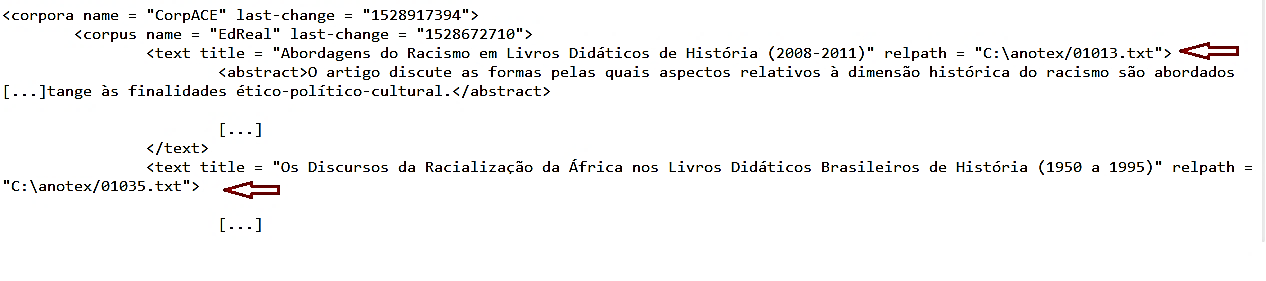
\includegraphics[width=\textwidth]{Fig13.png}
 \caption{Caminho relativo para localização dos textos.}
 \label{fig-13}
 \source{Adaptado pela autora do AnoTex v0.1b.}
\end{figure}

A análise dos dados coletados ratificou o entendimento inicial da pesquisa que a estrutura dos artigos científicos está condicionada à sua função social, uma vez que são eventos linguísticos caracterizados por um conjunto de propósitos comunicativos e por serem tipos relativamente estáveis de enunciados. As marcações em XML das representações de aspectos relacionados com o \textit{contexto de produção} do artigo científico podem influenciar a forma como o texto se organiza. Os elementos filtrados constitutivos dessas marcações revelam: emissor/enunciador, receptor/destinatário, lugar/instituição, suporte e conteúdo temático. Já da \textit{arquitetura geral} do gênero artigo que está relacionada ao gerenciamento do conteúdo do texto - a construção composicional característica do gênero - a princípio, são filtradas pelo AnoTex as capacidades discursivas do gênero compreendidas em três subdivisões, caracterizadas nas Figuras: 14 denominada Elementos \textit{Pré-textuais}, 15 denominada Elementos \textit{Textuais} e 16 denominada Elementos \textit{Pós-textuais}, a seguir:

\begin{enumerate}
    \item Elementos \textit{Pré-textuais} constantes do <front> como: periódico, título, autor, instituição, resumo e palavras-chave (\Cref{fig-14}).
\begin{figure}[htbp]
 \centering
 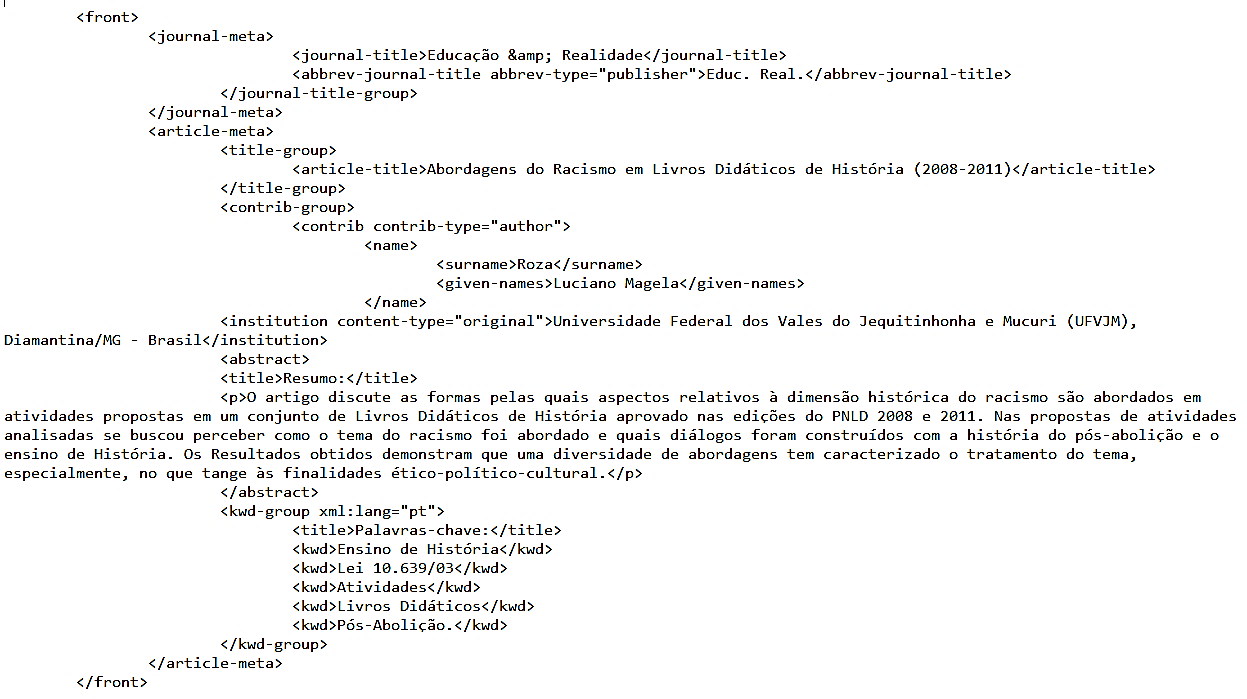
\includegraphics[width=\textwidth]{Fig14.png}
 \caption{Elementos Pré-textuais.}
 \label{fig-14}
 \source{Adaptado pela autora do \textit{CorpACE}.}
\end{figure}
    \item Elementos \textit{Textuais} constantes do <body> como: introdução, discussão e considerações finais (principais seções do artigo) (\Cref{fig-15}).
\begin{figure}[htbp]
\centering
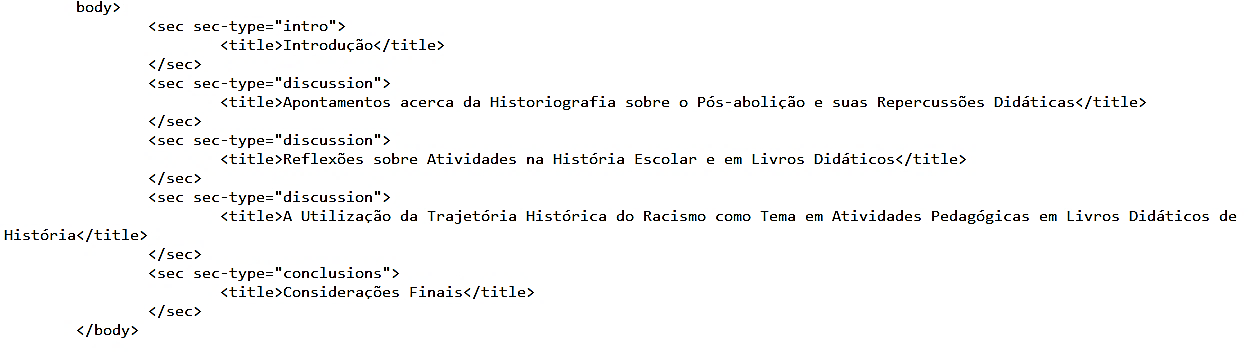
\includegraphics[width=\textwidth]{Fig15.png}
\caption{Elementos Textuais.}
\label{fig-15}
\source{Adaptado pela autora do \textit{CorpACE}.}
\end{figure}
    \item Elementos Pós-textuais constantes do <back> como: referências bibliográficas (\Cref{fig-16}).
\begin{figure}[htbp]
\centering
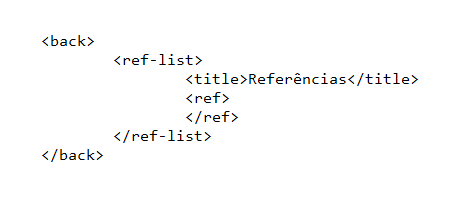
\includegraphics[width=0.85\textwidth]{Fig16.png}
\caption{Elementos Pós-textuais.}
\label{fig-16}
\source{Adaptado pela autora do \textit{CorpACE}.}
\end{figure}
\end{enumerate}

%Verificar se há erro no código de figura dentro da enumeração

Essa configuração do modelo computacional representativo para o gênero artigo científico enfatizado no uso de etiquetas XML permitiu destacar as características e a visualização das dimensões constitutivas do gênero, e delimitar os objetivos a serem atingidos em relação aos diferentes propósitos de seu uso. Além disso, essa representação arbórea dos elementos constitutivos do corpus pode dar pistas das características do gênero que podem ser mineradas e valoradas para o processamento do texto.

A indicação da localização e quantidade de ocorrências da filtragem dos elementos em negrito e itálico podem se tornar relevantes uma vez que os elementos mais conclusivos e significativos podem aparecer em páginas mais próximas da seção “introdução” (<sec sec-type="intro">) ou da seção “conclusão” (<sec sec-type="conclusions">) nos artigos científicos \cite{lin_identifying_1997}. Nesse caso, por meio da estrutura básica do gênero, poderia ser estabelecido um peso para o termo, observando-se a página onde ele ocorresse, além do número de vezes que ele fosse encontrado e marcado ao longo de todo artigo. Do ponto de vista linguístico, essa é uma informação que ainda precisa ser explorada na valoração do ranqueamento das sentenças.

\section{Conclusão}\label{sec-links}
Na medida em que foram analisadas, na prática, as marcações em XML (enriquecidas com informações linguísticas sobre a construção composicional do gênero, que indicam as relações entre elementos do contexto de produção e/ou da infraestrutura geral do texto-base), para o processamento do texto por ferramenta de PLN, foram verificadas algumas questões que confundiram a lógica do \textit{parsing} do AnoTex. Entretanto, a análise da maior parte dos dados coletados revelou que dentre os elementos que podem ser filtrados pelo AnoTex, e, que compuseram o \textit{CorpACE}, pode-se destacar uma estrutura básica do gênero artigo científico, constituída de elementos pré-textuais (<front>), textuais (<body>) e pós-textuais (<back>). Essa rigidez observada na estrutura da maioria dos 87 artigos coletados decorre exatamente da função do texto-base, que deve ser elaborado conforme normas preestabelecidas pelos periódicos, e, com fins e propósitos a que se destina, com o objetivo de garantir a comunicação da cientificidade do assunto abordado. O que ratifica o pressuposto de que a estrutura do gênero analisado é condicionada à sua função social.

Diante da análise sobre as ferramentas para anotação em \textit{corpus}, atualmente disponíveis, argumenta-se que essas não descrevem suficientemente as características do gênero textual base em combinação com um nível adequado de facilidade de uso. Uma vez que a principal finalidade da abordagem dessas ferramentas é a anotação morfossintática e semântica, ficou demonstrada uma lacuna na anotação da estrutura do gênero base. Sendo assim, é possível afirmar que há necessidade de uma estreita relação entre o sistema de anotação automática de texto com a análise do gênero do texto-base. E, por meio dessa abordagem, o AnoTex preenche uma importante lacuna no desenvolvimento das aplicações para a identificação e análise de dados estruturados representativos do gênero, de modo a proporcionar novas diretrizes na área de processamento de grandes quantidades de texto. Uma vez que os textos são eventos comunicativos carregados de propósitos, as decisões sobre as suas propriedades relevantes implicam reconhecer as propriedades da fonte, uma vez que estas são alimentadas por um conjunto de requisitos de propósitos comunicativos.
 
Outro ponto importante que merece ser destacado é que os esquemas de codificação precisam evoluir para atender novas demandas de maneira a não quebrar compatibilidade com versões antigas dos programas, e os programas precisam estar preparados para lidar com versões antigas dos dados possibilitando a compatibilidade retroativa. Entretanto, a língua natural, antes de ser representada/transformada em linguagem artificial, pelas marcações em XML por exemplo, deve ser entendida e normalizada, sob a pena de em alguns casos não favorecer a compatibilidade de interação.

A tecnologia deve ser abordada explorando os múltiplos conhecimentos necessários para o aperfeiçoamento das características linguísticas dos aplicativos com ênfase em PLN, ao invés da superespecialização. Só assim novos estudos serão abordados e, dentre eles, poderá existir uma possibilidade para a união de conhecimentos distintos, de forma a tornar mais eficientes a comunicação entre homens e máquinas. 

\printbibliography\label{sec-bib}
% if the text is not in Portuguese, it might be necessary to use the code below instead to print the correct ABNT abbreviations [s.n.], [s.l.]
%\begin{portuguese}
%\printbibliography[title={Bibliography}]
%\end{portuguese}


%full list: conceptualization,datacuration,formalanalysis,funding,investigation,methodology,projadm,resources,software,supervision,validation,visualization,writing,review
\begin{contributors}[sec-contributors]
\authorcontribution{Claudia Aparecida Fonseca}[conceptualization,formalanalysis,investigation,methodology,writing,review]
\authorcontribution{Marcus Vinícius Carvalho Guelpeli}[datacuration,formalanalysis,software,projadm,supervision,visualization]
\authorcontribution{Rafael Santiago de Souza Netto}[formalanalysis,software,visualization,writing]
\end{contributors}

\end{document}

